\documentclass{article}

\usepackage[preprint]{techreport}

\usepackage[utf8]{inputenc}
\usepackage[T1]{fontenc}
\usepackage[colorlinks=true,linkcolor=red,citecolor=green!50!black,urlcolor=blue]{hyperref}
\usepackage{url}
\usepackage{booktabs}
\usepackage{amsfonts}
\usepackage{amsmath}
\usepackage{amssymb}
\usepackage{nicefrac}
\usepackage{microtype}
\usepackage[table]{xcolor}
\usepackage{graphicx}
\usepackage{enumitem}
\usepackage{algorithm}
\usepackage{algpseudocode}
\usepackage{pifont}
\usepackage{multirow}
\usepackage{stfloats}
\usepackage{listings}
\usepackage{mdframed}
\usepackage{subcaption}
\usepackage{wrapfig}
\usepackage{fontawesome5}
\usepackage[skins,breakable]{tcolorbox}

\setlength{\textfloatsep}{10pt plus 2pt minus 2pt}
\setlength{\abovecaptionskip}{6pt}
\setlength{\belowcaptionskip}{2pt}

\definecolor{hlcol}{HTML}{FFF4CC}
\newcolumntype{g}{>{\columncolor{gray!15}}c}

\lstdefinestyle{promptstyle}{
  backgroundcolor=\color{gray!6},
  frame=single,
  rulecolor=\color{gray!45},
  basicstyle=\fontsize{7.5pt}{9pt}\selectfont\ttfamily,
  breaklines=true,
  breakatwhitespace=false,
  columns=fullflexible,
  keepspaces=true,
  showstringspaces=false,
  xleftmargin=6pt,
  xrightmargin=6pt,
  aboveskip=5pt,
  belowskip=5pt,
  captionpos=b,
}
\lstset{style=promptstyle}

\definecolor{boxaccent}{HTML}{4A7FB5}

% Intro highlight box: colored top rule + thin frame
\mdfdefinestyle{layerbox}{
  backgroundcolor=gray!3,
  linecolor=gray!35,
  linewidth=0.5pt,
  roundcorner=1.5pt,
  innerleftmargin=10pt,
  innerrightmargin=10pt,
  innertopmargin=8pt,
  innerbottommargin=8pt,
  skipabove=8pt,
  skipbelow=8pt,
  topline=true,
  splittopskip=12pt,
  frametitlebackgroundcolor=boxaccent!10,
}

% Design principle box: light accent background, no border
\mdfdefinestyle{principlebox}{
  backgroundcolor=boxaccent!4,
  linecolor=boxaccent!30,
  linewidth=0.4pt,
  roundcorner=1.5pt,
  innerleftmargin=9pt,
  innerrightmargin=9pt,
  innertopmargin=6pt,
  innerbottommargin=6pt,
  skipabove=4pt,
  skipbelow=4pt,
}

% Paper-style highlight box (parameterised accent colour)
\definecolor{princteal}{HTML}{2A9D8F}
\definecolor{princlavender}{HTML}{7B68AE}

\newtcolorbox{paperbox}[1][boxaccent]{
  enhanced, breakable,
  colback=#1!4,
  colframe=#1!22,
  boxrule=0.4pt,
  arc=1.5pt,
  left=10pt, right=10pt,
  top=8pt, bottom=8pt,
  borderline north={1.5pt}{0pt}{#1!55},
  before skip=6pt, after skip=6pt,
}

\customnotice{Technical Report. Work in progress, \href{https://github.com/HKUDS/DeepTutor}{latest codes}.}

\title{\raisebox{-0.2\height}{
\includegraphics[height=1.4em]{figures/logo.png}}\hspace{0.25em}DeepTutor: Towards Agentic Personalized Tutoring}

\author{
  Bingxi Zhao\textsuperscript{1,2}\thanks{Equal contribution.} \quad
  Jiahao Zhang\textsuperscript{1}$^*$ \quad
  Xubin Ren\textsuperscript{1} \quad
  Zirui Guo\textsuperscript{1} \\
  \bfseries Tianzhe Chu\textsuperscript{1} \quad
  Yi Ma\textsuperscript{1} \quad
  Chao Huang\textsuperscript{1}\thanks{Corresponding author.} \\[4pt]
  \textsuperscript{1}University of Hong Kong \qquad
  \textsuperscript{2}Beijing Jiaotong University \\
  \texttt{\{bingxizhao39, chaohuang75\}@gmail.com} \\[2pt]
  \faGithub~\url{https://github.com/HKUDS/DeepTutor}
}

\begin{document}

\maketitle

\begin{abstract}
% Education is one of the most promising real-world applications for Large Language Models (LLMs).
% However, conventional tutoring systems rely on static pre-training knowledge that lacks adaptation to individual learners, while existing RAG-augmented systems fall short in delivering personalized, guided feedback.
% To bridge this gap, we present \textsc{DeepTutor}, an agent-native open-source framework for personalized tutoring, where every tutoring feature shares a common personalization substrate.
% We propose a hybrid personalization engine that couples static knowledge grounding with a dynamic multi-resolution memory, distilling interaction history into a continuously evolving learner profile.
% Moreover, we construct a closed tutoring loop that bidirectionally couples citation-grounded problem solving with difficulty-calibrated question generation.
% The same personalization substrate further supports collaborative writing, multi-agent deep research, and interactive guided learning, enabling cross-modality coherence.
% To move beyond reactive interfaces, we introduce \textsc{TutorBot}, a proactive multi-agent layer that deploys tutoring capabilities through extensible skills and unified multi-channel access, providing a consistent experience across platforms.
% To better evaluate such a tutoring system, we construct \textsc{TutorBench}, a student-centric benchmark with source-grounded learner profiles, together with a first-person interactive protocol that measures adaptive tutoring from the learner's perspective.
% We further evaluate foundational agentic reasoning abilities across five authoritative benchmarks.
% Experiments show that \textsc{DeepTutor} improves personalized tutoring quality while maintaining general agentic reasoning abilities.
% We hope \textsc{DeepTutor} provides unique insights into next-generation tutoring systems for the community.
Education represents one of the most promising real-world applications for Large Language Models (LLMs). However, conventional tutoring systems rely on static pre-training knowledge that lacks adaptation to individual learners, while existing RAG-augmented systems fall short in delivering personalized, guided feedback. To bridge this gap, we present \textsc{DeepTutor}, an agent-native open-source framework for personalized tutoring where every feature shares a common personalization substrate. We propose a hybrid personalization engine that couples static knowledge grounding with dynamic multi-resolution memory, distilling interaction history into a continuously evolving learner profile. Moreover, we construct a closed tutoring loop that bidirectionally couples citation-grounded problem solving with difficulty-calibrated question generation. The personalization substrate further supports collaborative writing, multi-agent deep research, and interactive guided learning, enabling cross-modality coherence. To move beyond reactive interfaces, we introduce \textsc{TutorBot}, a proactive multi-agent layer that deploys tutoring capabilities through extensible skills and unified multi-channel access, providing consistent experience across platforms. To better evaluate such tutoring systems, we construct \textsc{TutorBench}, a student-centric benchmark with source-grounded learner profiles and a first-person interactive protocol that measures adaptive tutoring from the learner's perspective. We further evaluate foundational agentic reasoning abilities across five authoritative benchmarks. Experiments show that \textsc{DeepTutor} improves personalized tutoring quality while maintaining general agentic reasoning abilities. We hope \textsc{DeepTutor} provides unique insights into next-generation AI-powered and personalized tutoring systems for the community.
\end{abstract}

% ============================================================
\section{Introduction}
\label{sec:intro}
% ============================================================

Large language models have made open-ended educational dialogue practical, yet most deployed LLM tutors remain session-bounded assistants. They adapt to the immediate prompt rather than to a persistent learner model, and their functions are often implemented as isolated modules~\citep{chu-etal-2025-llm,letourneau2025systematicreviewaidriven}.
While a system may answer questions or generate exercises, these components share little state with one another. The result is not merely weaker personalization but a fragmented learning experience where pedagogical progress in one interaction rarely informs the next, as illustrated in Figure~\ref{fig:compare}.

Adopting a systems view, we argue that personalized tutoring requires a unified architecture rather than isolated prompts. This architecture must synchronize learner memory, task decomposition, and tool usage across multimodal sessions. Crucially, it should also provide a scalable framework for evolving from reactive to proactive support, obviating the need to rebuild the core runtime when introducing new interfaces or behaviors.

\begin{figure}[htbp]
    \centering
    
\includegraphics[width=\columnwidth]{figures/compare-0411.png}
    \caption{Comparison between prior LLM products with \textsc{DeepTutor}. Conventional LLM tutors rely on generic priors, producing answers or exercises that may mismatch the learner's syllabus and proficiency, while \textsc{DeepTutor} grounds both problem solving and question generation in the learner's knowledge base and diagnosed weaknesses.}
    \label{fig:compare}
\end{figure}

Agent-Native Design. The agentic paradigm~\citep{yao2023reactsynergizingreasoningacting,wang2024survey} is uniquely suited to this challenge for three reasons.
First, agents can maintain persistent state across extended horizons, which is essential for cultivating a dynamic learner model rather than treating interactions as isolated events.
For instance, a tutoring agent can diagnose recurring misconceptions, such as a student's persistent confusion between the chain and product rules, and adaptively refine its instructional strategy when relevant topics re-emerge in future sessions.
Second, agents can orchestrate tools and sub-agents into structured workflows, enabling complex tasks like problem-solving, targeted exercise generation, and guided learning to be implemented as systematic pipelines rather than brittle prompt chains.
Third, the underlying agent infrastructure provides a scalable foundation for autonomous operation, allowing proactive behaviors to extend the system’s utility without re-engineering its core logic.
Consequently, we architect \textsc{DeepTutor} along two complementary dimensions: \emph{personalized agentic tutoring}, which establishes the core pipelines and the unifying personalization engine, and \emph{proactive autonomous companionship}, which leverages those pipelines for long-term, cross-platform engagement.
\begin{itemize}[leftmargin=*]
\item \textbf{Personalized Agentic Tutoring.}\quad
A hybrid personalization engine synthesizes static knowledge grounding with a dynamic \emph{trace forest}, distilling interaction history into a continuously refined learner profile.
We establish a closed-loop pedagogy that interlocks citation-grounded problem solving with difficulty-calibrated question generation. This shared substrate further powers collaborative writing, multi-agent deep research, and interactive guided learning, ensuring that pedagogical progress transcends individual modalities.

\item \textbf{Proactive Autonomous Companionship.}\quad
Through \textsc{TutorBot}, \textsc{DeepTutor} operationalizes its tutoring core into autonomous agents equipped with extensible skills, multi-bot coordination, and context-preserving multi-channel gateways.
This architecture transforms the system from a reactive interface into a proactive companion capable of autonomously initiating review sessions, synthesizing daily practice, and remediating diagnosed knowledge gaps across platforms.
\end{itemize}

This report presents \textsc{DeepTutor}, an open-source framework that actualizes this vision. The system is built upon a unified runtime where personalization, context propagation, and event-based streaming are natively shared across all workflows, spanning both reactive tutoring and proactive deployment. We offer this two-dimensional design as a generalizable blueprint for architecting personalized tutoring systems that seamlessly evolve into context-aware, proactive agents.

To evaluate the system’s core, we construct \textsc{TutorBench}, a student-centric benchmark comprising university-level materials across five diverse disciplines. Each entry synthesizes a source-grounded learner profile with diagnosed knowledge gaps and a corresponding interactive tutoring task. A first-person student simulator conducts multi-turn dialogues to rigorously assess adaptive pedagogical behaviors from the learner's perspective. 
In this report, we focus our quantitative evaluation on the foundational tutoring pipeline while characterizing cognitive extensions and \textsc{TutorBot} as system components whose long-term efficacy warrants extended longitudinal studies.

Our main contributions are as follows:
\begin{itemize}[nosep,leftmargin=*]
\item We propose \textsc{DeepTutor}, a novel intelligent tutoring framework that decouples a validated pedagogical core (\emph{personalized agentic tutoring}) from its deployment-oriented extensions (\emph{proactive autonomous companionship}), both anchored by a unified personalization engine.
\item We introduce a dynamic multi-resolution memory architecture that distills multi-turn interaction history into a continuously refined learner profile, enabling a tightly coupled bidirectional loop between problem solving and personalized question generation.
\item We design \textsc{TutorBot}, a proactive multi-agent layer that operationalizes tutoring capabilities through extensible skills, multi-agent coordination, and context-unified access across multiple platforms.
\item We construct \textsc{TutorBench}, a student-centric benchmark featuring a first-person interactive protocol to assess adaptive pedagogy. Empirical results demonstrate that \textsc{DeepTutor} improves personalized tutoring quality by 10.8\% over the strongest baseline, while simultaneously achieving an average 28.6\% gain in general reasoning across five backbone models on standard benchmarks.
\end{itemize}
% ============================================================
\section{Related Work}
\label{sec:related}
% ============================================================

\paragraph{Tool-Augmented LLM Agents.}
The evolution from monolithic LLM prompting to tool-augmented reasoning has been swift.
Early work demonstrated that language models can learn to invoke external APIs through supervised fine-tuning~\citep{schick2024toolformer}, while subsequent frameworks interleaved explicit thought and action traces to enable dynamic, multi-step tool use~\citep{yao2023reactsynergizingreasoningacting}.
Recent advances have expanded the planning horizon of such agents, from hierarchical sub-goal decomposition~\citep{zhao2025llmbasedagenticreasoningframeworks,wu-etal-2025-agentic,li2025intheflowagenticoptimizationeffective} to long-horizon research pipelines that maintain coherent state across many reasoning steps~\citep{chen2026iterresearch}.
A common thread, however, is that these agents operate in bounded episodes: they begin, reason, and conclude within a single session.
Tutoring, by contrast, is an inherently \emph{longitudinal} endeavor that spans weeks or months and benefits from an evolving model of the individual learner, a requirement that existing agentic frameworks do not directly address.

\paragraph{Personalization and Memory in LLMs.}
Endowing language models with persistent, user-specific memory is an active research front.
Dialogue-level approaches employ reflective summarization to compress past conversations into reusable context~\citep{tan-etal-2025-prospect}, while user-modeling methods accumulate structured preferences and attributes across sessions~\citep{li-etal-2025-hello,cho-etal-2022-personalized}.
At the retrieval layer, RAG-based personalization injects user-relevant documents into the generation context~\citep{li2025surveypersonalizationragagent,guo2025raganythingallinoneragframework}, and workflow-induction techniques distill recurring behavioral patterns into reusable agent plans~\citep{wang2024agentworkflowmemory}.
Architecturally, hierarchical memory systems such as MemGPT~\citep{packer2023memgpt}, HiMem~\citep{qin2025himem}, and G-Memory~\citep{yang2025gmemory} organize information at multiple temporal scales.
In the education domain specifically, learner modeling has a long history through knowledge tracing, evolving from Bayesian formulations~\citep{corbett1994knowledge} to neural architectures~\citep{piech2015deep,zhang2017dkvmn,ghosh2020akt}.
We build on both traditions with a tree-structured dynamic memory called the \emph{trace forest}, designed specifically for tutoring. Unlike flat conversation logs or fixed-size summaries, the trace forest preserves interaction history at multiple resolutions and feeds back into both problem solving and question generation.

\paragraph{AI for Education.}
The application of LLMs to education has generated a rich and rapidly growing literature.
Recent work spans conversational tutoring with explicit student modeling~\citep{park2024empoweringpersonalizedlearning}, multi-agent pedagogical architectures~\citep{wang2025llmpoweredmultiagentframeworkgoaloriented}, open-source tutoring platforms~\citep{xu2025opentutorai}, conversational learning diagnosis~\citep{chen2026parld}, knowledge-tracing-augmented recommendation~\citep{liu2025tutorllm}, and pedagogically aligned optimization of tutor behavior~\citep{dinucujianu2025pedagogy}.
Benchmarks such as MathTutorBench~\citep{huang2025mathtutorbench} have advanced the measurement of open-ended pedagogical quality, yet most evaluations still adopt an instructor-centric view that treats the student as a generic receiver of instruction.
Our work differs in two respects.
First, we unify multiple tutoring modalities, including problem solving, question generation, writing, research, and guided learning, through a single, continuously evolving learner model rather than treating each as an independent capability.
Second, we evaluate the resulting system from the \emph{student's} perspective, using first-person simulated dialogues grounded in individualized learner profiles rather than relying on instructor-defined rubrics alone.

\section{DeepTutor Architecture}
\label{sec:overview}

Engineering a personalized tutoring system necessitates a fundamental shift from session-constrained assistants to persistent, agentic companions.
Current architectures often suffer from dimensional silos:
traditional agents demonstrate multi-step reasoning yet lack persistent learner states; personalization engines accumulate history but remain decoupled from active tutoring pipelines; and educational platforms adapt to isolated prompts without a shared substrate to propagate context across diverse tasks and channels.

\textsc{DeepTutor} synthesizes these fragmented capabilities into a unified architectural design. In this section, we first articulate the core design principles that anchor the system around cross-functional personalization (\S\ref{sec:principles}). We then detail the agent-native infrastructure that enables tutoring workflows and proactive agency to coexist and collaborate within a single, composable runtime (\S\ref{sec:infrastructure}).


\subsection{Design Principles}
\label{sec:principles}
A robust personalized tutoring system must be \textit{pedagogically deep} to model individual learners, \textit{functionally broad} to span diverse knowledge modalities, and \textit{architecturally open} to accommodate emerging interfaces and autonomous behaviors. While addressing these demands in isolation is straightforward, the primary challenge lies in integrating them without letting the architecture degenerate into a fragmented collection of point solutions. We consolidate these requirements into three guiding design principles.

\paragraph{Principle 1: Shared Personalization as the Unifying Substrate.}
Systems often treat problem-solving, question generation, and research as decoupled states, causing the tutor to lose pedagogical context when a learner switches tasks. \textsc{DeepTutor} mitigates this by routing all workflows through a centralized personalization engine—comprising shared knowledge bases, the \emph{trace forest}, and a unified learner profile $\mathcal{D}$. Consequently, a weakness identified during problem-solving directly shapes the subsequent guided session, while insights from research refine the parameters of future question generation. The learner interacts with a cohesive, evolving intelligence rather than a fragmented toolkit.
\paragraph{Principle 2: Reusable Agentic Workflows over Monolithic Features.}
Architectures that hard-code pedagogical behaviors are inherently brittle and scale poorly. We instead adopt an agent-native design where tutoring functions—from writing assistance to deep research—are implemented as composable workflows atop a shared runtime for retrieval, reasoning, and personalization. Because these workflows inherit standardized context-propagation and delivery mechanisms by construction, extending the system with new modalities does not require re-engineering the underlying stack.
\paragraph{Principle 3: Proactive Agency with Unified Context.}
Autonomy provides value only if the learner’s state remains coherent across all entry points. In \textsc{DeepTutor}, proactive behavior is an architectural extension of the tutoring substrate rather than a separate product surface. The tutoring dimension formalizes the learner model and workflows, while the proactive dimension leverages them for autonomous, multi-platform engagement. Our objective is autonomy without context fragmentation: whether a student solves a problem via a web interface or receives a review reminder via Telegram, they engage with a singular, context-unified tutor.

\subsection{Agent-Native Infrastructure}
\label{sec:infrastructure}

The design principles articulated above dictate a core implementation requirement: every workflow and interaction entry point must operate within a unified, shared runtime. This subsection details how \textsc{DeepTutor}’s infrastructure operationalizes this requirement to ensure architectural consistency.

\paragraph{Common Runtime for Extensible Workflows. }To avoid redundant implementation across diverse interfaces or pedagogical tasks, \textsc{DeepTutor} centers execution on a uniform runtime that provides a suite of foundational services: retrieval-augmented generation (RAG), agentic reasoning, sandboxed code execution, memory access, and multi-agent orchestration. All tutoring behaviors—ranging from multi-stage problem solving to parallel deep research—are implemented as composable workflows atop this layer. By design, these workflows inherit standardized context-propagation mechanisms and a unified streaming protocol, ensuring functional parity across the system.
\paragraph{Unified Context and Event-Driven Streaming. }A system-wide context structure encapsulates the complete state of each interaction turn, including session metadata, conversation history, tool registries, knowledge-base references, and the personalization signal $\mathcal{C}_{\text{mem}}$. This ensures that every agent, regardless of its specific entry point, operates on a coherent and synchronized learner model. Furthermore, all agent outputs are emitted as strongly-typed events via an asynchronous event bus. This decouples the core agent logic from the delivery layer, enabling diverse consumers to consume and render the same telemetry stream without custom adaptation.
\paragraph{Convergent Entry Points. }A critical architectural consequence of this design is that every entry point including the web interface, CLI, programmatic SDK, and \textsc{TutorBot}~(\S\ref{sec:proactive}) converges on a single orchestrator. This convergence ensures that both the reactive tutoring pipelines and the proactive autonomous components described in the subsequent sections execute on the identical infrastructure, anchored by the same continuously evolving learner model.



% % ------------------------------------------------------------
% \subsection{Agent-Native Infrastructure}
% \label{sec:infrastructure}
% % ------------------------------------------------------------

% The three principles above impose a concrete implementation requirement: every workflow and every entry point must share the same runtime.
% This subsection describes how \textsc{DeepTutor}'s infrastructure realizes that requirement.

% \paragraph{Shared Runtime for Extensible Workflows.}
% Rather than reimplementing functionality for each interface or learning task, \textsc{DeepTutor} centers execution on a uniform runtime that provides retrieval, reasoning, code execution, memory access, and orchestration as common services.
% All tutoring behaviors, from multi-stage problem solving to parallel deep research, are realized as reusable workflows over this layer and inherit the same context propagation and streaming protocol.

% \paragraph{Unified Context and Streaming.}
% A unified context structure encapsulates each turn's complete state, including session identity, conversation history, enabled tools, knowledge-base references, and the personalization context $\mathcal{C}_{\text{mem}}$.
% This ensures that every agent, regardless of entry point, operates on the same personalization signal.
% All agent output is emitted as typed events through an asynchronous event bus, decoupling agent logic from delivery and enabling any consumer, whether a web frontend, CLI, or messaging bot, to render the same stream without modification.

% \paragraph{Convergent Entry Points.}
% This design has a critical architectural consequence: every entry point, whether the web interface, CLI, programmatic SDK, or TutorBot~(\S\ref{sec:proactive}), converges on the same orchestrator and streams through the same event protocol.
% The tutoring and proactive components described in the following sections therefore execute on the same infrastructure and are personalized by the same evolving learner model.

% ============================================================
\section{Personalized Agentic Tutoring}
\label{sec:responsive}
% ============================================================

\begin{figure*}[t]
    \centering
    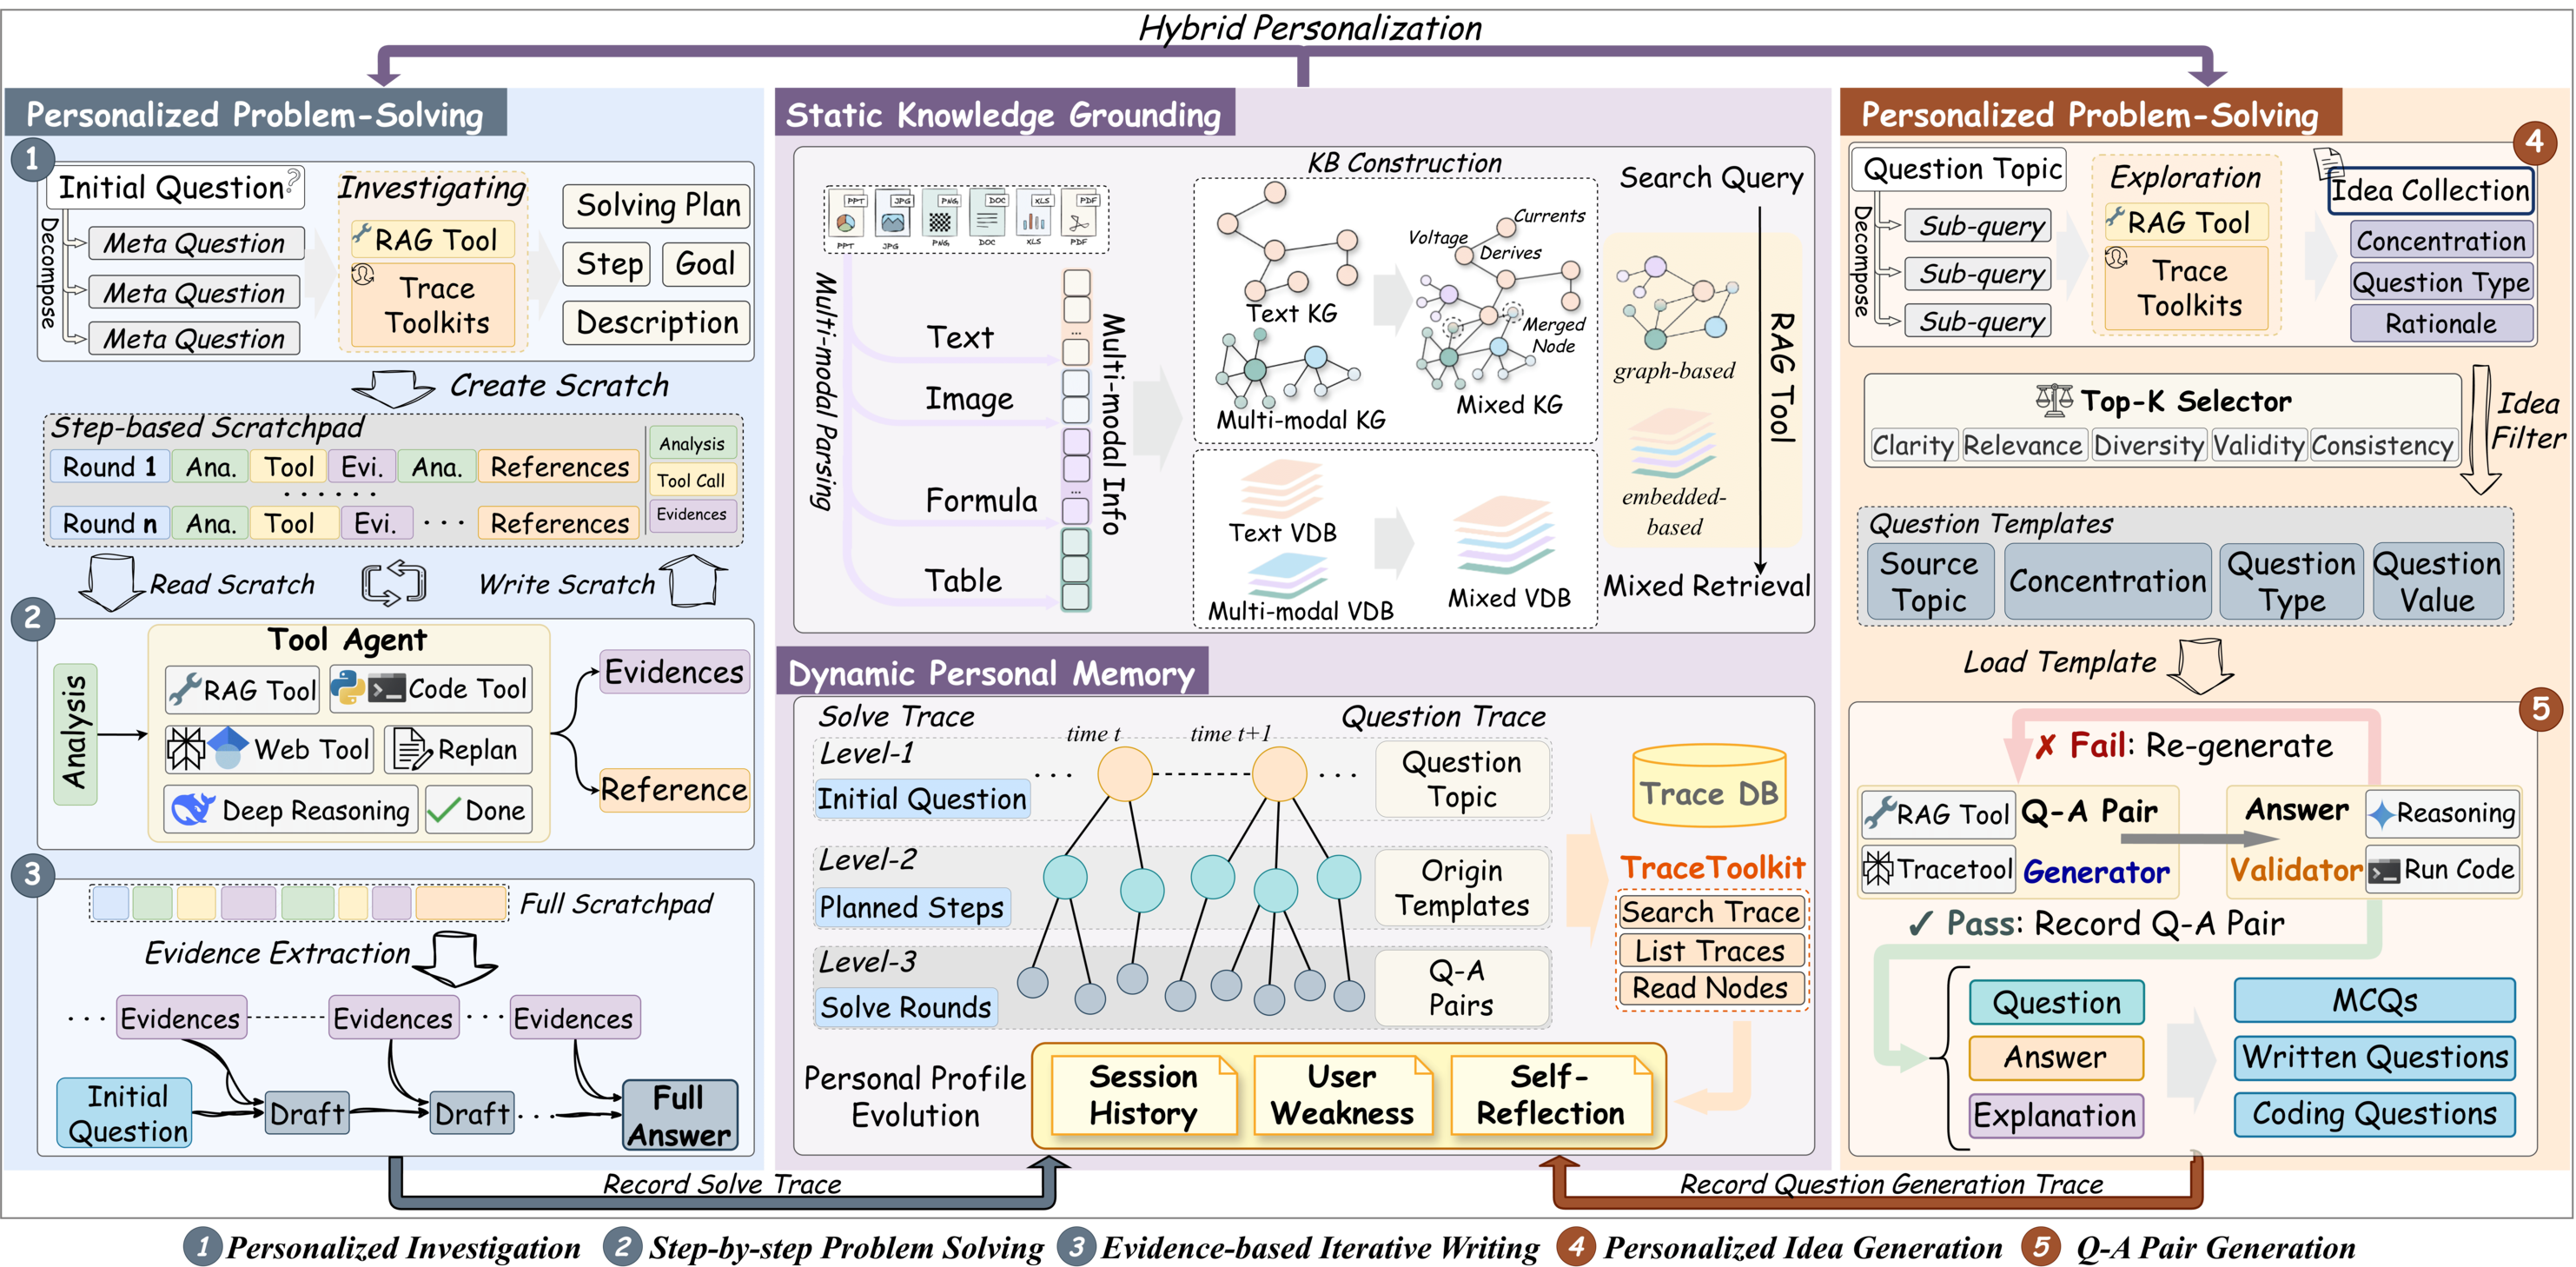
\includegraphics[width=\textwidth]{figures/full-pipe-0316.png}
    \caption{Overview of the personalization substrate and the foundational tutoring loop.
    A hybrid engine fuses static knowledge grounding (center) with dynamic personal memory (bottom).
    Problem solving (left, stages \ding{172}--\ding{174}) and question generation (right, stages \ding{175}--\ding{176}) form a closed cycle: both pipelines read from and write back to the shared learner profile.}
    \label{fig:overview}
\end{figure*}

An agentic tutoring system must do far more than answer isolated questions.
Learners solve problems, generate targeted practice, express understanding through writing, synthesize information from diverse sources, and absorb new concepts through structured engagement.
When these modalities are supported independently, the result is a disconnected toolkit: the writing agent forgets what the problem solver just diagnosed, and the question generator ignores what the learner struggled with yesterday.
Unifying all capabilities under a single, continuously evolving understanding of the individual learner is the organizing principle of this section.

\S\ref{sec:personalization} describes the personalization substrate.
\S\ref{sec:loop} presents the foundational tutoring loop coupling problem solving with question generation.
\S\ref{sec:cognitive_ext} extends this loop along three complementary dimensions of knowledge work.

% ===========================================================================
\subsection{The Personalization Substrate}
\label{sec:personalization}
% ===========================================================================

Effective tutoring demands two complementary forms of context: \emph{domain expertise} (what the course teaches) and \emph{learner awareness} (how the individual student has engaged with that material).
Domain knowledge tells the system what is important; learner awareness tells it what is important \emph{for this student, right now}.
The personalization engine supplies both through a static knowledge-grounding module and a dynamic personal memory, whose outputs are fused before every agent step.

\subsubsection{Static Knowledge Grounding}
\label{sec:rag}

Course materials are decomposed into atomic content units and indexed through two complementary structures~\citep{wang2024mineruopensourcesolutionprecise}.
A \emph{knowledge graph} $\mathcal{G}$ captures structural and conceptual relations among definitions, theorems, and examples, while dense encoders project all units into an \emph{embedding index} $\mathcal{B}$~\citep{guo2025raganythingallinoneragframework}.
The rationale for dual indexing is that educational queries span a continuum from structurally precise questions such as ``What are the prerequisites of Stokes' theorem?'' to semantically diffuse ones such as ``I'm confused about the relationship between circulation and flux.''
Graph traversal over $\mathcal{G}$ excels at the former, while dense search over $\mathcal{B}$ handles the latter.
The two candidate sets are fused via reciprocal rank fusion~\citep{cormack2009reciprocal}, deduplicated, and truncated to a context budget, yielding the domain grounding $\mathcal{C}_{\text{rag}}$.

\subsubsection{Dynamic Personal Memory: The Trace Forest}
\label{sec:memory}

Whereas static grounding captures \emph{what is taught}, dynamic memory captures \emph{how the individual has learned}.
The central representational challenge is how to remember months of tutoring interactions in a form that is simultaneously compact enough to fit in a context window and rich enough to inform future pedagogy.

We address this with the \emph{Trace Forest}~$\mathcal{F}$, a hierarchical, multi-resolution data structure in which each tree records one complete tutoring interaction as a semantically searchable artifact.
Nodes are organized into three levels of granularity.
\emph{Level~1} stores session-level metadata and a global summary, capturing the overall topic, outcome, and duration of the interaction.
\emph{Level~2} captures intermediate planning units produced during task decomposition, each recording a sub-goal, its status, and a condensed rationale.
\emph{Level~3} preserves fine-grained execution records, including tool outputs, retrieved evidence, and validation outcomes.
Every node carries a dense embedding computed from its textual content, enabling similarity-based retrieval across the entire forest~\citep{packer2023memgpt,qin2025himem,yang2025gmemory}.

A new trace tree is created at the end of each tutoring session.
The three-level structure is populated incrementally as the session progresses: the planner creates Level~2 nodes when it decomposes a problem, the executor appends Level~3 nodes as it processes each sub-goal, and a post-session summarizer generates the Level~1 root from the completed tree.

The multi-resolution design reflects a deliberate trade-off between flat conversation logs (easy to store but expensive to search) and fixed-size summaries (compact but detail-lossy).
The three-level hierarchy allows the system to operate at the right resolution for each task: session summaries for long-range trends, planning-level nodes for conceptual trajectories, and execution-level nodes for recalling exactly \emph{how} a student arrived at a particular misunderstanding.

Rather than treating $\mathcal{F}$ as a passive archive, we expose it through a programmatic \emph{TraceToolkit} with three operations:
\textsc{SearchTrace} performs semantic retrieval across all trees and levels, ranking nodes by embedding similarity to the current query and returning results with their ancestry paths so that fine-grained nodes can be interpreted in the context of their parent session.
\textsc{ListTraces} supports filtered enumeration by time range, topic, or outcome, enabling agents to quickly survey recent activity or locate sessions on a particular subject.
\textsc{ReadNodes} provides full-content access to one or more nodes together with ancestry-path reconstruction, allowing an agent to drill down from a session summary to the exact execution record that produced a specific misconception diagnosis.
This toolkit is available to every agent in the system, making past interactions a first-class resource that can be consulted as readily as the knowledge base itself.

\subsubsection{Profile Construction and Injection}
\label{sec:injection}

Three specialized memory agents process each new trace in parallel, each maintaining one dimension of the learner profile $\mathcal{D} = (\mathcal{D}_s, \mathcal{D}_w, \mathcal{D}_r)$:
\begin{itemize}[nosep,leftmargin=*]
\item \textbf{Session History} $\mathcal{D}_s$: a running account of topics covered and performance trends.
The session-history agent extracts the subject, difficulty level, and outcome of each session and appends a dated entry to $\mathcal{D}_s$, enabling downstream agents to identify long-range patterns such as topics that recur frequently or performance trajectories that plateau.
\item \textbf{Weakness Diagnosis} $\mathcal{D}_w$: a prioritized inventory of knowledge gaps, each labeled as \emph{active} or \emph{resolved}.
The weakness agent examines execution-level nodes for evidence of confusion, incorrect reasoning steps, or repeated errors, and either creates a new gap entry or updates an existing one.
A gap is labeled \emph{resolved} when the student demonstrates correct application across at least two subsequent sessions; it reverts to \emph{active} if later evidence shows the misconception has resurfaced.
\item \textbf{Self-Reflection} $\mathcal{D}_r$: the system's pedagogical self-critique, consisting of actionable notes on what explanatory strategies worked well and what to improve.
The reflection agent compares the tutor's intended approach with the student's actual responses, noting instances where scaffolding was too sparse or too dense, where analogies succeeded or confused, and where the pacing mismatched the learner's readiness.
\end{itemize}

The three-dimensional decomposition is motivated by a pedagogical observation: effective tutoring requires knowing not only \emph{what} the student has done ($\mathcal{D}_s$) and \emph{where they struggle} ($\mathcal{D}_w$), but also \emph{how the tutor itself should adapt} ($\mathcal{D}_r$).
This self-reflective dimension is rare in existing systems; most treat the tutor as a fixed function of the student profile, ignoring the possibility that the tutoring strategy itself should evolve.

Before each agent step, a personalization context $\mathcal{C}_{\text{mem}}$ is assembled through two complementary channels.
First, \emph{active trace retrieval} uses the TraceToolkit to surface the most relevant nodes from $\mathcal{F}$, with retrieval budget allocated proportionally across the three levels.
Second, \emph{role-specific profile excerpting} routes different slices of $\mathcal{D}$ to different agents: the planner receives $\mathcal{D}_s$ and $\mathcal{D}_w$ to inform investigation strategy, the writer receives $\mathcal{D}_r$ to calibrate tone and depth, and the idea agent receives $\mathcal{D}_w$ to target practice at diagnosed gaps.
This selective injection prevents context saturation while ensuring that each agent receives precisely the personalization signal it needs.

% ===========================================================================
\subsection{Closing the Tutoring Loop}
\label{sec:loop}
% ===========================================================================

A personalization substrate is only as valuable as the feedback loop that keeps it current.
The foundational tutoring loop couples two complementary pipelines, problem solving and question generation, through the shared learner model.

\paragraph{Why two pipelines, and why coupled?}
A tutor that only answers questions never challenges the student's blind spots; a system that only generates practice is an exercise book, not a tutor.
Coupling the two makes the system pedagogically complete: weaknesses diagnosed during problem solving propagate to $\mathcal{D}_w$ and shape which questions are generated next, while the learner's performance on those questions refines $\mathcal{D}_s$ and $\mathcal{D}_r$, improving future explanations.

\paragraph{Personalized Problem Solving.}
The problem-solving pipeline separates concerns that compete for the same context window into three sequential agent stages.
\emph{Stage~\ding{172}, Personalized Investigation}, decomposes the student's question into meta-questions, gathers evidence from both $\mathcal{C}_{\text{rag}}$ and $\mathcal{C}_{\text{mem}}$, and synthesizes a solving plan tailored to the individual's gaps.
This ensures that personalization enters the pipeline at the earliest possible stage rather than being retrofitted during writing.
\emph{Stage~\ding{173}, Step-by-Step Solving}, executes each sub-goal through a think--act--observe loop~\citep{yao2023reactsynergizingreasoningacting} with self-notes and hierarchical compression to manage context growth, plus adaptive replanning when evidence reveals the current plan is inadequate.
\emph{Stage~\ding{174}, Evidence-Based Writing}, constructs the final answer through iterative draft--refine passes, using the learner profile $\mathcal{D}$ to calibrate depth and tone.
Beginners receive scaffolded derivations~\citep{wood1976role}, while proficient learners receive concise insights.
Every claim carries a traceable citation to retrieved evidence.

The rationale for this three-stage decomposition is that investigation, execution, and presentation serve fundamentally different cognitive functions and compete for the same limited context budget.
Prior approaches that fold all three into a single reasoning loop~\citep{yao2023reactsynergizingreasoningacting,wu-etal-2025-agentic} sacrifice either investigation depth or presentation quality as the problem grows complex.

\paragraph{Personalized Question Generation.}
Question generation is decomposed into two stages that separate \emph{what to ask} from \emph{how to ask and verify}.
\emph{Stage~\ding{175}, Idea Generation}, maps the conceptual landscape around a topic through the lens of the individual learner, producing candidate question ideas with personalized rationales grounded in diagnosed gaps from $\mathcal{D}_w$.
An evaluator-driven filtering-then-ranking pass prunes ill-formed or redundant candidates.
\emph{Stage~\ding{176}, Critic-Guided Generation}, instantiates each idea into a question--answer--explanation triple, verified by a structurally separated validator that checks template alignment, factual correctness, and, for computational questions, sandboxed code execution.
Because the validator shares no reasoning chain with the generator, it must independently verify correctness, reducing self-confirming errors~\citep{spiliopoulou2025playfavorites}.

\paragraph{The Closed-Loop Dynamic.}
\label{sec:cycle}
After each interaction, the system appends a new trace tree to $\mathcal{F}$ and the three memory agents update $\mathcal{D}$ in parallel.
The key property is \emph{bidirectional task coupling}: the solving pipeline feeds the generation pipeline through $\mathcal{D}_w$, and the generation pipeline feeds back into the solving pipeline through $\mathcal{D}_s$ and $\mathcal{D}_r$.
Because every agent can query the trace forest at any time, this feedback extends beyond profile-level summaries to fine-grained precedents from any prior interaction, enabling increasingly nuanced personalization as the interaction history grows.
The complete closed-loop algorithm is provided in Appendix~\ref{app:algorithm}.

% ===========================================================================
\subsection{Beyond Q\&A: Cognitive Extension across Knowledge Modalities}
\label{sec:cognitive_ext}
% ===========================================================================

\begin{figure}[t]
    \centering
    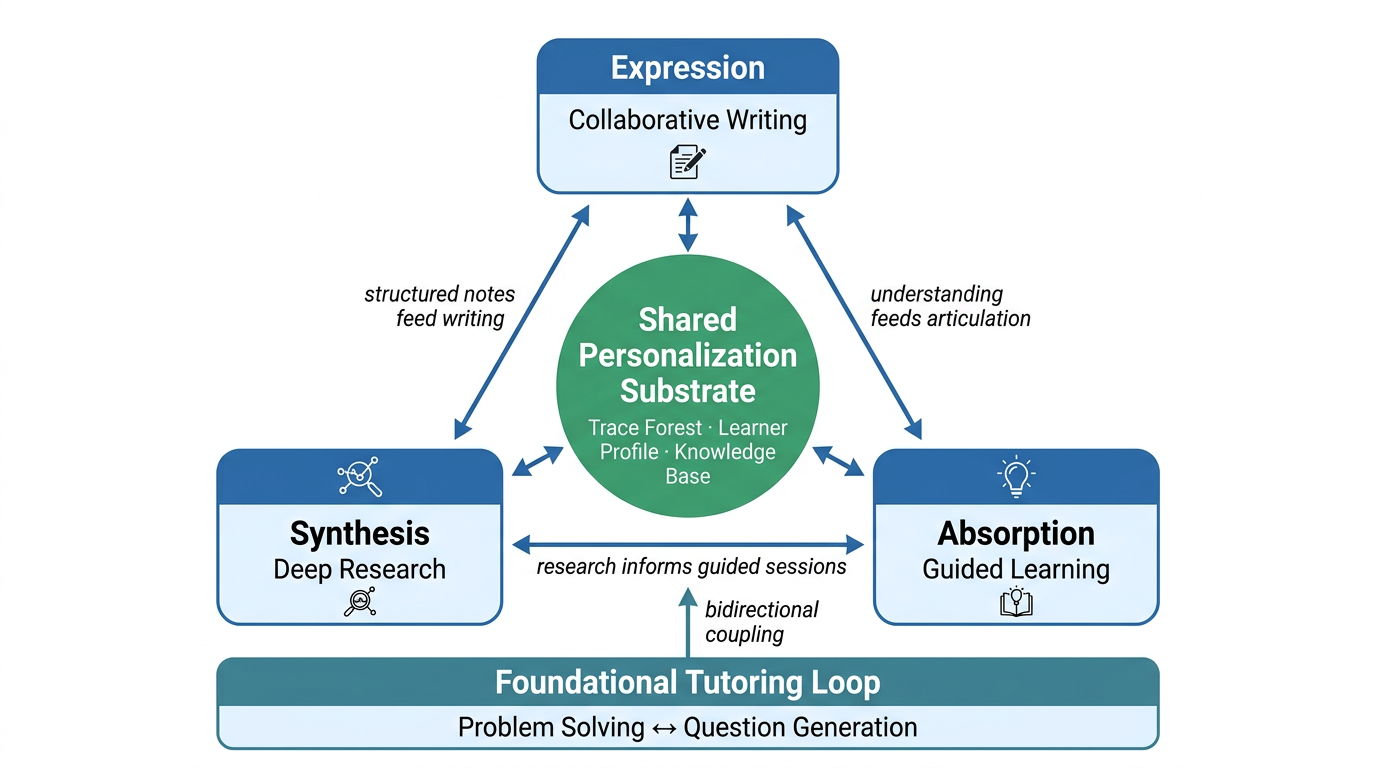
\includegraphics[width=\columnwidth]{figures/cognitive-extension.png}
    \caption{Three cognitive extensions, \emph{expression}, \emph{synthesis}, and \emph{absorption}, extend the tutoring loop into a broader support cycle. All three share the same personalization substrate, so progress in any modality informs the others.}
    \label{fig:extension}
\end{figure}

The tutoring loop of~\S\ref{sec:loop} covers the most familiar form of learning, but real learning extends beyond asking and answering.
Learners also \emph{express} understanding through writing, \emph{synthesize} information from diverse sources, and \emph{absorb} new concepts through active engagement (Figure~\ref{fig:extension}).
The key design question is how to support these modalities without fragmenting the learner's experience; our answer is to run every extension on the same personalization substrate.

\paragraph{Knowledge Expression: Collaborative Writing.}
An \texttt{EditAgent} operates in a tool-augmented loop: given a document context and an editing instruction, it retrieves relevant passages via RAG, gathers supplementary information through web search when needed, and produces structured edits with inline citations.
Access to $\mathcal{C}_{\text{mem}}$ lets it calibrate assistance to the individual, providing scaffolded guidance for beginners and concise refinements for advanced writers.
Every writing session generates a trace that captures the topics chosen and the structural weaknesses encountered, enriching the learner profile for all downstream capabilities.

\paragraph{Knowledge Synthesis: Multi-Agent Deep Research.}
When learners move from coursework to independent study, they need to construct knowledge by integrating information from many sources, a task that demands multi-step agentic orchestration rather than single-turn generation.
The deep research capability addresses this through a four-stage multi-agent pipeline.
First, the user's query is rephrased and decomposed into topics.
Multiple \texttt{ResearchAgent} instances then operate concurrently, each drawing on the full tool suite including knowledge-base retrieval, web search, academic paper search, and sandboxed code execution.
A manager agent dynamically injects emergent sub-topics discovered during investigation, allowing the research to follow threads that were not anticipated at decomposition time.
Finally, the pipeline generates output in one of four modes, \emph{comprehensive}, \emph{focused}, \emph{comparative}, or \emph{exploratory}, reflecting distinct cognitive needs. A student surveying a new field needs landscape notes rather than a lengthy report, while a student choosing between two frameworks needs a comparative analysis rather than an exhaustive survey.

\paragraph{Knowledge Absorption: Interactive Guided Learning.}
Problem solving and research are student-initiated; guided learning inverts this dynamic by having the system lead the learner through structured, active engagement, a mode shown to dramatically outperform passive reading~\citep{freeman2014active}.
The capability is realized through a three-agent pipeline.
A \texttt{DesignAgent} creates a structured learning plan calibrated to diagnosed weak points from $\mathcal{D}_w$, identifying key concepts, prerequisite relationships, common misconceptions, and an appropriate difficulty progression.
An \texttt{InteractiveAgent} then leads the student through the plan via Socratic multi-turn dialogue, introducing concepts progressively, posing probing questions, and providing scaffolded hints rather than direct answers.
After the session, a \texttt{SummaryAgent} generates a synthesis of knowledge points covered and areas for follow-up, enriching the trace forest for all future interactions.

\paragraph{Cross-Modality Coherence.}
Because all three modalities share the same trace forest and learner profile, they form a mutually reinforcing cycle without explicit cross-modality wiring.
Weaknesses surfaced during problem solving inform guided sessions; insights from guided learning improve research strategies; and structured notes from deep research feed back into writing assistance.

% ============================================================
\section{Proactive Tutoring}
\label{sec:proactive}
% ============================================================

\begin{figure*}[t]
    \centering
    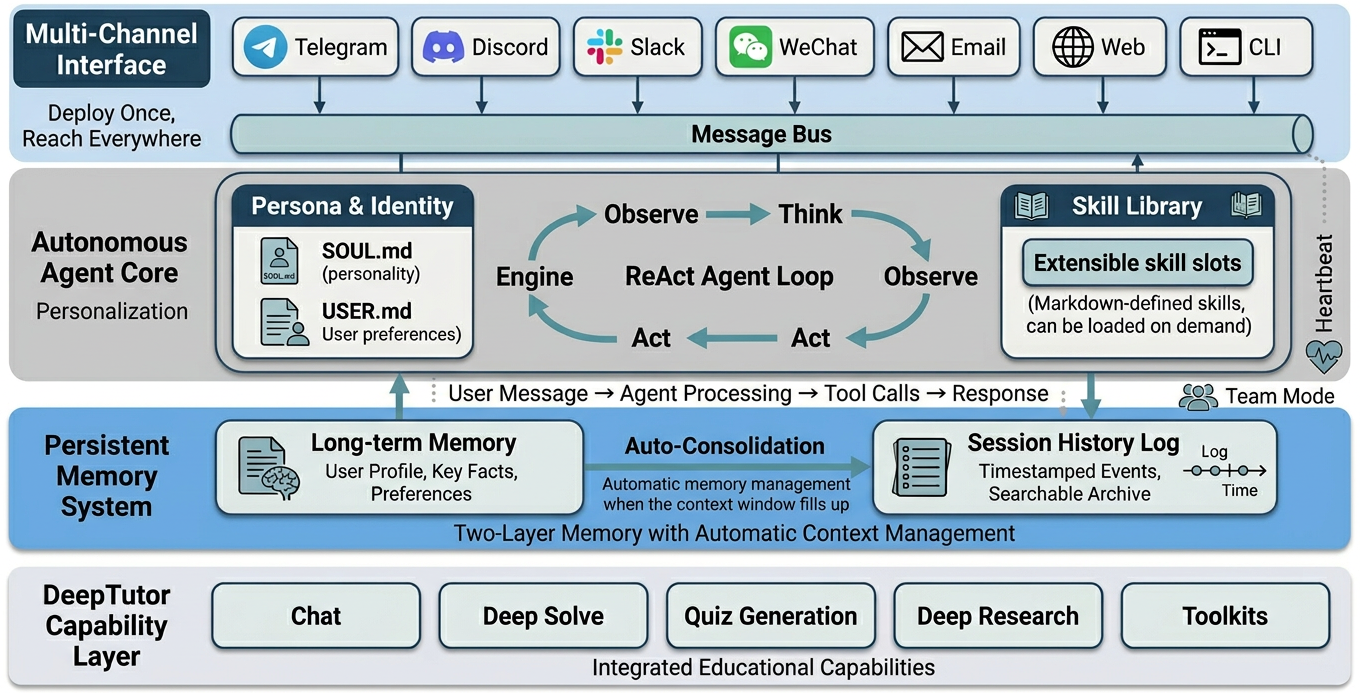
\includegraphics[width=\textwidth]{figures/tutorbot.png}
    \caption{TutorBot architecture. Four layers from top to bottom: a \emph{multi-channel interface} connecting twelve messaging platforms through a unified bus; an \emph{autonomous agent core} with a customizable persona (Soul) and extensible skills; a \emph{persistent memory system} with automatic consolidation; and the \emph{shared DeepTutor runtime} exposing the full tutoring stack as reusable services.}
    \label{fig:tutorbot}
\end{figure*}

The personalized tutoring capabilities described in~\S\ref{sec:responsive}, however comprehensive, remain largely learner-initiated.
They are typically accessed through a web interface or CLI, which means the learner must decide when to engage and which entry point to use.

This creates two practical limitations.
First, \emph{interaction friction}: the learner must remember to return, open the right interface, and formulate the next request.
Second, \emph{context fragmentation}: a student who uses the web interface on a laptop, the CLI from a terminal, and a messaging app on a phone can easily end up with disconnected sessions that do not share state.

TutorBot is our design for this proactive layer.
Rather than introducing a second tutoring system, it reuses the tutoring workflows described in~\S\ref{sec:responsive} in a longer-horizon, multi-channel setting.
This section describes four design decisions, illustrated in Figure~\ref{fig:tutorbot}: enabling each bot to autonomously invoke the existing tutoring workflows through a persistent agent loop~(\S\ref{sec:agentloop}), extending behavior through skills~(\S\ref{sec:skills}), supporting multiple specialized bots in parallel~(\S\ref{sec:multibot}), and unifying context across channels~(\S\ref{sec:channels}).

% ------------------------------------------------------------
\subsection{From Capability Execution to Autonomous Agency}
\label{sec:agentloop}
% ------------------------------------------------------------

The first requirement is that every workflow available in the tutoring dimension, including problem solving, question generation, collaborative writing, deep research, and guided learning, must be invocable by an autonomous bot, not only by a human clicking a button.

TutorBot achieves this through runtime reuse: it invokes the same tutoring workflows that power the web interface, through the same orchestrator and personalization backbone.
An adapter layer translates between the bot's conversational message format and \textsc{DeepTutor}'s unified context structure.
Each TutorBot instance runs in-process within the \textsc{DeepTutor} server, sharing the same LLM configuration, knowledge-base indices, and provider connections, with no separate deployment required.
The CLI exposes bot management as a first-class entry point, and bot-initiated conversations flow through the same pipeline as web or messaging interactions.

At the core of each instance is an autonomous agent loop (Algorithm~\ref{alg:tutorbot} in Appendix~\ref{app:tutorbot}) following the observe--think--act paradigm (cf.\ Figure~\ref{fig:tutorbot}, center).
Each inbound message triggers three phases: \emph{context assembly} weaves conversation history, persona definition, skill descriptions, and long-term memory into the agent's working state; \emph{reasoning} invokes tools iteratively until the problem is resolved or a budget is exhausted; and \emph{dispatch} sends the response back through the originating channel.

Two design choices distinguish this loop from a standard ReAct agent.
First, \textbf{persistent two-layer memory} (cf.\ Figure~\ref{fig:tutorbot}, bottom-left): TutorBot maintains a long-term user profile alongside a searchable session history log.
An automatic consolidation mechanism monitors context-window pressure and distills the oldest messages into both layers before the window overflows, enabling coherent interactions across arbitrarily long trajectories.
Second, \textbf{high-level tutoring actions} (cf.\ Figure~\ref{fig:tutorbot}, bottom): beyond low-level primitives, TutorBot can invoke complete tutoring services such as RAG-grounded explanation, deep reasoning, sandboxed code execution, and academic paper search as first-class actions within its reasoning loop.

% ------------------------------------------------------------
\subsection{Unbounded Extensibility via Skills}
\label{sec:skills}
% ------------------------------------------------------------

The tutoring capabilities cover a broad range of learning tasks, but a proactive agent must also support workflow-specific behaviors that are not appropriate to hard-code into the core loop, such as study scheduling, repository monitoring, or recurring report generation.

TutorBot achieves this extensibility through \emph{skills}, self-contained declarative modules that extend the bot's repertoire without modifying core code (cf.\ Figure~\ref{fig:tutorbot}, right).
Each skill is a natural-language specification comprising four elements: \emph{triggers} that tell the agent when to activate the skill, step-by-step \emph{instructions} guiding the agent's behavior, a declaration of the \emph{tools} required, and optional executable \emph{scripts} for complex operations.
Skills function as curriculum for the agent: they teach the LLM how to combine its existing tools in new ways, much as a human tutor might learn a new teaching technique by reading a pedagogical guide.

Built-in skills bridge TutorBot to the full tutoring stack, including problem solving, question generation, deep research, knowledge-base management, and learner memory, while utility skills extend it with scheduling, summarization, and document management.
Skills are loaded from two sources, with workspace-level overrides taking precedence over built-in defaults to enable per-bot customization.

A \emph{skill-creator} meta-skill further allows the bot to author new skills at runtime: when a recurring workflow is not covered by the existing library, the bot can propose, create, and install a new skill.
This mechanism keeps the proactive layer open-ended without requiring frequent modifications to the underlying infrastructure.

% ------------------------------------------------------------
\subsection{Collective Intelligence via Multi-Bot Parallelism}
\label{sec:multibot}
% ------------------------------------------------------------

Complex learning scenarios, from exam preparation to multi-faceted research, benefit from parallel specialized agents.
A single \textsc{DeepTutor} deployment can host multiple independent TutorBot instances, each with its own persona, skill configuration, proactive schedule, and conversation history, while all bots share the same knowledge bases and tutoring runtime.

\paragraph{Personality and Specialization via Soul Templates.}
Each bot's identity, including communication style, expertise scope, and behavioral constraints, is defined through structured \emph{Soul templates} (cf.\ Figure~\ref{fig:tutorbot}, left).
A registry of pre-built templates enables rapid instantiation of specialized agents such as a patient math tutor, a research assistant, a language practice partner, or an exam preparation coach.
Specialization goes beyond surface-level persona: a math tutor bot foregrounds problem-solving and question-generation skills, while a research assistant bot prioritizes literature synthesis and summarization.
The learner thus interacts with a team of specialized agents, each optimized for a particular cognitive task.

\paragraph{Proactive Autonomy.}
Each bot runs a heartbeat service that periodically wakes the agent to evaluate whether proactive action is warranted, for instance checking whether the student has completed a scheduled review, whether a daily practice problem should be generated based on active weaknesses, or whether new papers added to the knowledge base merit summarization.
The LLM itself decides whether to act or defer, reducing unnecessary activations while allowing the system to initiate follow-up when the learner may benefit from it.
A scheduling service supports one-time, recurring, and cron-expression-based tasks that the bot can create dynamically, enabling it to adapt its proactive cadence to the learner's rhythm.

\paragraph{Self-Evolution.}
Because each bot operates in a mutable workspace, it can modify its own configuration over time.
The memory consolidator continuously refines the bot's understanding of the student, the skill-creator produces new behaviors in response to emergent needs, and the proactive schedule adapts to engagement patterns.
Each bot therefore evolves independently, acquiring new skills, refining its persona, and adjusting its proactive cadence, all without affecting other bots in the same deployment.

% ------------------------------------------------------------
\subsection{Unified Context across Channels and Devices}
\label{sec:channels}
% ------------------------------------------------------------

TutorBot embodies a ``deploy once, reach everywhere'' principle: a single bot instance connects to twelve channel adapters spanning consumer messaging (Telegram, Discord, WhatsApp, QQ), enterprise platforms (Slack, Feishu, DingTalk, WeCom), open protocols (Matrix, Email), and self-hosted solutions (MoChat), all behind a unified message bus.

More importantly, all channels share the same backend context.
A student who uses the web interface in the morning, the CLI in the afternoon, and Telegram in the evening interacts with one continuous thread: the same trace forest, learner profile, and personalization context span all entry points.

\paragraph{Discussion.}
The four design dimensions of the proactive layer, namely autonomous capability composition, skill-based extensibility, multi-bot parallelism, and unified cross-channel context, define how the same personalized tutoring capabilities can be deployed in longer-horizon settings.
Our claim is not that this layer is fully evaluated in the present report, but that it provides a concrete systems design for extending a validated tutoring core into proactive, context-unified agents.
We view this as one of the primary insights that a technical report format allows us to share: a detailed architectural blueprint that can inform future implementations and evaluations.

% ============================================================
\section{Evaluation}
\label{sec:evaluation}
% ============================================================

This section evaluates two tightly scoped contributions of \textsc{DeepTutor}.
First, we introduce a \textbf{student-centric benchmark and first-person interactive protocol} intended to measure tutoring quality from the learner's perspective rather than from the instructor's alone.
Second, we evaluate the \textbf{foundational tutoring pipeline}, including problem solving, question generation, and the shared personalization engine, which constitutes the experimentally validated core of the system.

We evaluate along three complementary axes.
\emph{First-person interactive evaluation}~(\S\ref{sec:interactive_eval}) probes adaptive personalization through simulated multi-turn student dialogues.
\emph{General problem-solving transfer}~(\S\ref{sec:generalization}) tests whether the tutoring-oriented pipeline decomposition strengthens the backbone's reasoning ability on standard benchmarks.
\emph{Component-level ablation}~(\S\ref{sec:ablation}) isolates the individual contribution of each architectural pillar.

% ===========================================================================
\subsection{TutorBench: A Student-Centric Benchmark}
\label{sec:tutorbench}
% ===========================================================================

Existing educational benchmarks predominantly adopt an instructor-centric perspective, treating the student as a generic receiver of instruction~\citep{chu-etal-2025-llm,kurdi2020systematic}.
\textsc{TutorBench} closes this gap: every entry couples a detailed learner persona with source-grounded knowledge gaps and an interactive tutoring task, placing the student at the center of evaluation.

\begin{figure*}[t]
  \centering
  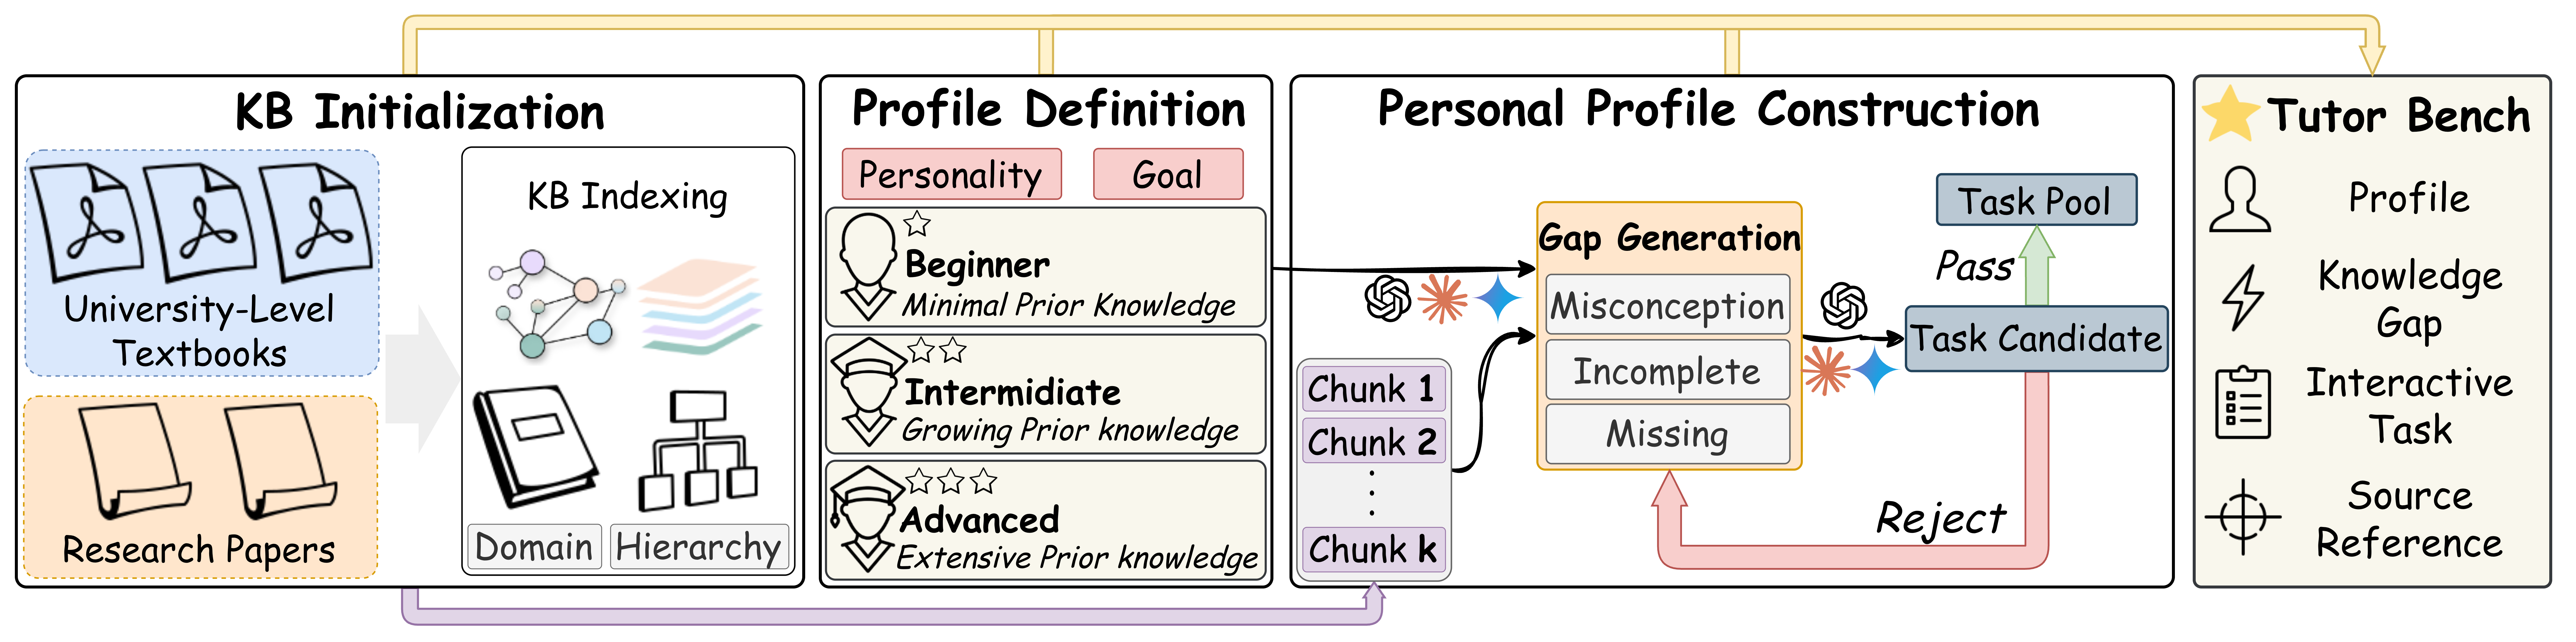
\includegraphics[width=\textwidth]{figures/bench-0315.png}
  \caption{Construction pipeline of \textsc{TutorBench}. Each entry contains a learner profile, source-grounded knowledge gaps, and an interactive tutoring task.}
  \label{fig:datagen}
\end{figure*}

\paragraph{Construction Pipeline.}
University-level textbooks and research papers are first indexed into the dual-representation knowledge base~(\S\ref{sec:rag}), from which a domain hierarchy is derived.
Each knowledge base instantiates three learner profiles at the \emph{beginner}, \emph{intermediate}, and \emph{advanced} levels, which differ in educational background, learning purpose, and per-topic mastery states.
For each profile, source-grounded knowledge gaps are generated across three types: \emph{misconceptions}, \emph{incomplete understanding}, and \emph{missing knowledge}~\citep{smith1993misconceptions,shute2008focus}.
These gaps are assembled into interactive tasks via rejection sampling that verifies gap coherence, task--gap alignment, and conversational naturalness.
All generated entries undergo human review for factual correctness, profile plausibility, and pedagogical soundness.

\paragraph{Statistics.}
\textsc{TutorBench} draws on 30 knowledge bases spanning five disciplines (humanities, sciences, engineering, business, and frontier research), instantiating 90 learner profiles and 270 interactive tasks.
Every entry carries three source-grounded knowledge gaps anchored to specific passages from the underlying materials.

% ===========================================================================
\subsection{First-Person Interactive Evaluation}
\label{sec:interactive_eval}
% ===========================================================================

Building on rubric-based LLM evaluation~\citep{zheng2023judging,huang2025mathtutorbench} and simulated-student paradigms~\citep{dinucujianu2025pedagogy,scarlatos2026simulatedstudents,pan2025tutorup}, we design a first-person interactive evaluation protocol (Figure~\ref{fig:evaluation}; Appendix~\ref{app:eval:simulator}) in which an LLM-based student simulator, initialized from a \textsc{TutorBench} entry with knowledge gaps rendered as first-person belief statements, engages each tutoring system in multi-turn dialogue.
The resulting transcripts are then scored by an independent LLM judge against personalized rubrics.

\paragraph{Metrics.}
Tutoring quality is assessed along ten dimensions, each scored on a 1--5 Likert scale.
Five \textbf{solve-side} metrics capture explanation quality: \emph{Source Faithfulness}~(SF), \emph{Personalization}~(PER), \emph{Applicability}~(APP), \emph{Vividness}~(VID), and \emph{Logical Depth}~(LD).
Five \textbf{practice-side} metrics capture question quality: \emph{Fitness}~(FIT), \emph{Groundedness}~(GND), \emph{Diversity}~(DIV), \emph{Answer Quality}~(ANS), and \emph{Cross Concept}~(CC).
Detailed rubric definitions appear in Appendix~\ref{app:eval:rubrics}.

\paragraph{Protocol.}
We use \emph{Gemini-3-Flash} to power both the student simulator and all tutor backbones, while \emph{Claude Sonnet~4.6} serves as the judge at temperature zero.
Each transcript is scored three times and averaged to reduce variance.
Results are obtained on the full \textsc{TutorBench} release consisting of 270 tasks across 90 profiles and 30 knowledge bases.

\paragraph{Baselines.}
To disentangle the contribution of our pipeline design from that of the backbone model, we construct four representative baselines within a unified evaluation harness that shares the same RAG tool and backbone:
\emph{Naive Tutor} (direct prompting),
\emph{CoT Tutor} (chain-of-thought~\citep{wei2022chain}),
\emph{Self-Refine Tutor} (draft followed by a pedagogical review pass~\citep{madaan2024selfrefine}), and
\emph{ReAct Tutor} (think--act--observe loop~\citep{yao2023reactsynergizingreasoningacting}).

{%
\setlength{\aboverulesep}{0pt}%
\setlength{\belowrulesep}{0pt}%
\renewcommand{\arraystretch}{1.18}%
\begin{table*}[t]
\centering
\small
\resizebox{\textwidth}{!}{%
\setlength{\tabcolsep}{4.2pt}
\begin{tabular}{l ccccc g ccccc g cc}
\toprule
& \multicolumn{6}{c}{\textbf{Solve Quality}}
& \multicolumn{6}{c}{\textbf{Practice Quality}}
& \multicolumn{2}{c}{\textbf{Overall}} \\
\cmidrule(lr){2-7} \cmidrule(lr){8-13} \cmidrule(lr){14-15}
\textbf{System}
  & SF & PER & APP & VID & LD & \textit{Avg}
  & FIT & GND & DIV & ANS & CC & \textit{Avg}
  & OQ & $\Delta$\% \\
\midrule
Naive Tutor
  & 3.22 & 4.24 & 4.44 & 3.89 & 3.99 & 3.96
  & 3.20 & 2.46 & 2.83 & 3.87 & 3.12 & 3.10
  & 3.53 & \textcolor{gray}{--} \\
CoT Tutor
  & 3.34 & 4.22 & 4.47 & 3.82 & 4.01 & 3.97
  & 3.18 & 2.50 & 2.79 & 3.81 & 3.04 & 3.06
  & 3.52 & {-0.28\%} \\
Self-Refine Tutor
  & 3.28 & 4.28 & \textbf{4.61} & 3.94 & 4.14 & 4.05
  & 3.17 & 2.49 & 2.88 & 3.88 & 2.97 & 3.08
  & 3.57 & {+1.13\%} \\
ReAct Tutor
  & \underline{3.35} & 4.37 & 4.40 & 3.70 & 3.96 & 3.96
  & 3.16 & 2.47 & 2.75 & \underline{3.94} & 3.07 & 3.08
  & 3.52 & {-0.28\%} \\
\midrule
\textsc{DeepTutor}
  & \textbf{3.36} & \textbf{4.59} & 4.56 & 4.81 & \textbf{4.61} & \textbf{4.39}
  & \textbf{3.35} & \textbf{2.96} & \textbf{3.44} & \textbf{3.98} & \textbf{3.38} & \textbf{3.42}
  & \textbf{3.91} & \textcolor{teal!80!black}{\textbf{+10.76\%}} \\
\quad w/o Memory
  & \textbf{3.36} & 4.22 & 4.57 & \textbf{4.83} & 4.52 & \underline{4.30}
  & 3.15 & \underline{2.80} & \underline{3.34} & 3.90 & \underline{3.31} & \underline{3.30}
  & \underline{3.80} & \textcolor{teal!80!black}{\textbf{+7.65\%}} \\
\quad w/o RAG
  & 3.11 & \underline{4.41} & 4.55 & \textbf{4.83} & \underline{4.53} & 4.29
  & \underline{3.31} & 2.23 & 3.30 & 3.84 & 3.19 & 3.17
  & 3.73 & \textcolor{teal!80!black}{\textbf{+5.67\%}} \\
\quad w/o RAG + Memory
  & 3.16 & 4.17 & \underline{4.60} & \underline{4.82} & 4.48 & 4.25
  & 3.25 & 2.22 & 3.27 & 3.85 & 3.14 & 3.15
  & 3.70 & \textcolor{teal!80!black}{\textbf{+4.82\%}} \\
\bottomrule
\end{tabular}}
\caption{Main results on \textsc{TutorBench}. Upper block: baselines. Lower block: \textsc{DeepTutor} with ablation variants. \textit{Avg}~is the group mean; OQ~is the \underline{O}verall \underline{Q}uality across all ten metrics; $\Delta$\%~is relative improvement over the Naive Tutor baseline. All metrics are 1--5~$\uparrow$. \textbf{Bold}~=~best; \underline{underline}~=~second best.}
\label{tab:interactive_all}
\end{table*}
}

\paragraph{Results.}
Table~\ref{tab:interactive_all} reveals a striking pattern: the four baselines cluster within a narrow performance band despite employing substantially different reasoning strategies, suggesting that reasoning sophistication alone does not translate into better personalization.
\textsc{DeepTutor} breaks out of this band, achieving an overall quality improvement of 10.76\% over the strongest baseline.

On the solve side, \emph{Vividness} sees the largest lift (+0.87 over the best baseline), reflecting the multi-stage pipeline's ability to produce structurally richer explanations with embedded examples and visual cues.
\emph{Personalization} and \emph{Logical Depth} follow, indicating that the system successfully diagnoses individual gaps and scaffolds logically grounded reasoning chains.
On the practice side, the advantage is even more pronounced.
\emph{Groundedness} records the largest absolute gain, benefiting directly from RAG-grounded question generation, while \emph{Diversity} and \emph{Cross Concept} profit from the structured learner history that guides the idea agent toward novel angles and inter-concept connections.

\paragraph{Cross-Domain Generalization.}
Decomposing results by discipline (Appendix~\ref{app:results}), solve-side quality remains broadly stable across all five domains, suggesting that the trace-forest-driven learner model generalizes well.
Practice-side quality shows somewhat more variation, reflecting inherent differences in question structure across disciplines, such as the relative difficulty of generating well-grounded multiple-choice distractors in humanities versus engineering.

% ===========================================================================
\subsection{General Problem-Solving Ability}
\label{sec:generalization}
% ===========================================================================

A natural concern is that a pipeline optimized for personalized tutoring might sacrifice general reasoning ability.
We test this directly by evaluating \textsc{DeepTutor}'s problem-solving pipeline, with the personalization engine disabled, on five established benchmarks spanning STEM reasoning (HLE~\citep{phan2025hle}, GPQA-Diamond~\citep{rein2024gpqa}, LiveBench~\citep{white2025livebench}), agentic problem solving (GAIA~\citep{mialon2024gaia}), and long-context reasoning (AA-LCR~\citep{artificialanalysis2025lcr}).
To ensure a fair comparison, all base model were also evaluated using our open-sourced pipeline, which may differ slightly from the self-reported scores in the official report.\footnote{See \url{https://github.com/HKUDS/DeepTutor/tree/eval} for full codes.}

{%
\setlength{\aboverulesep}{0pt}%
\setlength{\belowrulesep}{0pt}%
\renewcommand{\arraystretch}{1.18}%
\begin{table*}[t]
\centering
\small
\resizebox{\textwidth}{!}{%
\setlength{\tabcolsep}{5pt}
\begin{tabular}{l ccc cccc c c}
\toprule
& \multicolumn{3}{c}{\textbf{STEM Reasoning}} & \multicolumn{4}{c}{\textbf{General Agent (GAIA)}} & \textbf{Long Ctx} & \\
\cmidrule(lr){2-4} \cmidrule(lr){5-8} \cmidrule(lr){9-9}
\textbf{Pass@1} & HLE$^*$ & GPQA-D$^{**}$ & LiveBench$^{***}$ & L1 & L2 & L3 & Overall$^\dagger$ & AA-LCR & \textit{Avg~$\Delta$} \\
\midrule
Gemini-3-Flash & 19.40 & 81.31 & 70.00 & 43.40 & 40.70 & 15.38 & 37.58 & 63.00 & \multirow{2}{*}{\textcolor{teal!80!black}{\textbf{+29.12\%}}} \\
\quad+\textsc{DeepTutor} & \textbf{30.80} & \textbf{84.85} & \textbf{96.00} & \textbf{56.60} & \textbf{50.00} & \textbf{23.08} & \textbf{47.88} & \textbf{74.67} & \\
\midrule
Sonnet-4.5 & 8.40 & 72.22 & 64.33 & 37.74 & 30.23 & 7.69 & 29.09 & 53.33 & \multirow{2}{*}{\textcolor{teal!80!black}{\textbf{+32.03\%}}} \\
\quad+\textsc{DeepTutor} & \textbf{14.60} & \textbf{73.23} & \textbf{82.00} & \textbf{50.94} & \textbf{48.84} & \textbf{23.08} & \textbf{45.45} & \textbf{54.00} & \\
\midrule
Qwen-3.5-Plus & 16.80 & 88.38 & 69.00 & 44.23 & 35.71 & 13.64 & 33.94 & 66.00 & \multirow{2}{*}{\textcolor{teal!80!black}{\textbf{+23.00\%}}} \\
\quad+\textsc{DeepTutor} & \textbf{24.20} & 87.88 & \textbf{93.00} & \textbf{50.94} & \textbf{53.49} & \textbf{32.00} & \textbf{49.09} & \textbf{69.67} & \\
\midrule
GPT-5-Mini & 16.46 & 80.81 & 71.00 & 32.08 & 30.23 & 7.69 & 27.27 & 68.67 & \multirow{2}{*}{\textcolor{teal!80!black}{\textbf{+27.11\%}}} \\
\quad+\textsc{DeepTutor} & \textbf{21.20} & 80.30 & \textbf{93.00} & \textbf{54.72} & \textbf{52.33} & \textbf{26.92} & \textbf{49.09} & \textbf{71.00} & \\
\midrule
Minimax-M2.5 & 14.00 & 82.83 & 59.30 & 35.29 & 22.78 & 12.00 & 23.64 & 66.00 & \multirow{2}{*}{\textcolor{teal!80!black}{\textbf{+31.50\%}}} \\
\quad+\textsc{DeepTutor} & \textbf{19.40} & \textbf{83.33} & \textbf{73.00} & \textbf{52.94} & \textbf{44.30} & \textbf{32.00} & \textbf{42.42} & \textbf{76.40} & \\
\bottomrule
\end{tabular}}
\caption{General problem-solving \textbf{pass@1 scores} across five backbone models.
Each pair of rows compares the bare backbone against the same backbone augmented with \textsc{DeepTutor}'s pipeline.
$^*$We utilize a fixed subset with 500-questions.
$^{**}$GPQA-Diamond.
$^{***}$We use the reasoning subset.
$^\dagger$GAIA scores are reported per difficulty level (L1--L3).}
\label{tab:generalization}
\end{table*}
}

As shown in Table~\ref{tab:generalization}, all five backbone families benefit substantially when augmented with \textsc{DeepTutor}'s pipeline, with an average gain of 28.6\% across benchmarks.
The improvements are particularly pronounced on harder tasks such as GAIA Level~3 and HLE, where the investigate-before-plan design helps contain error accumulation in long reasoning chains.

Note that the baselines here are bare backbone models without tool access, so the gains reflect the combined effect of the multi-stage pipeline \emph{and} the tool suite it orchestrates.
The ablation in~\S\ref{sec:ablation} provides the complementary view by holding the pipeline constant and removing individual components.
Together with Table~\ref{tab:interactive_all}, these results confirm that the foundational pipeline improves both personalized tutoring and general agentic reasoning.

% ===========================================================================
\subsection{Ablation Study}
\label{sec:ablation}
% ===========================================================================

\begin{figure}[t]
  \centering
  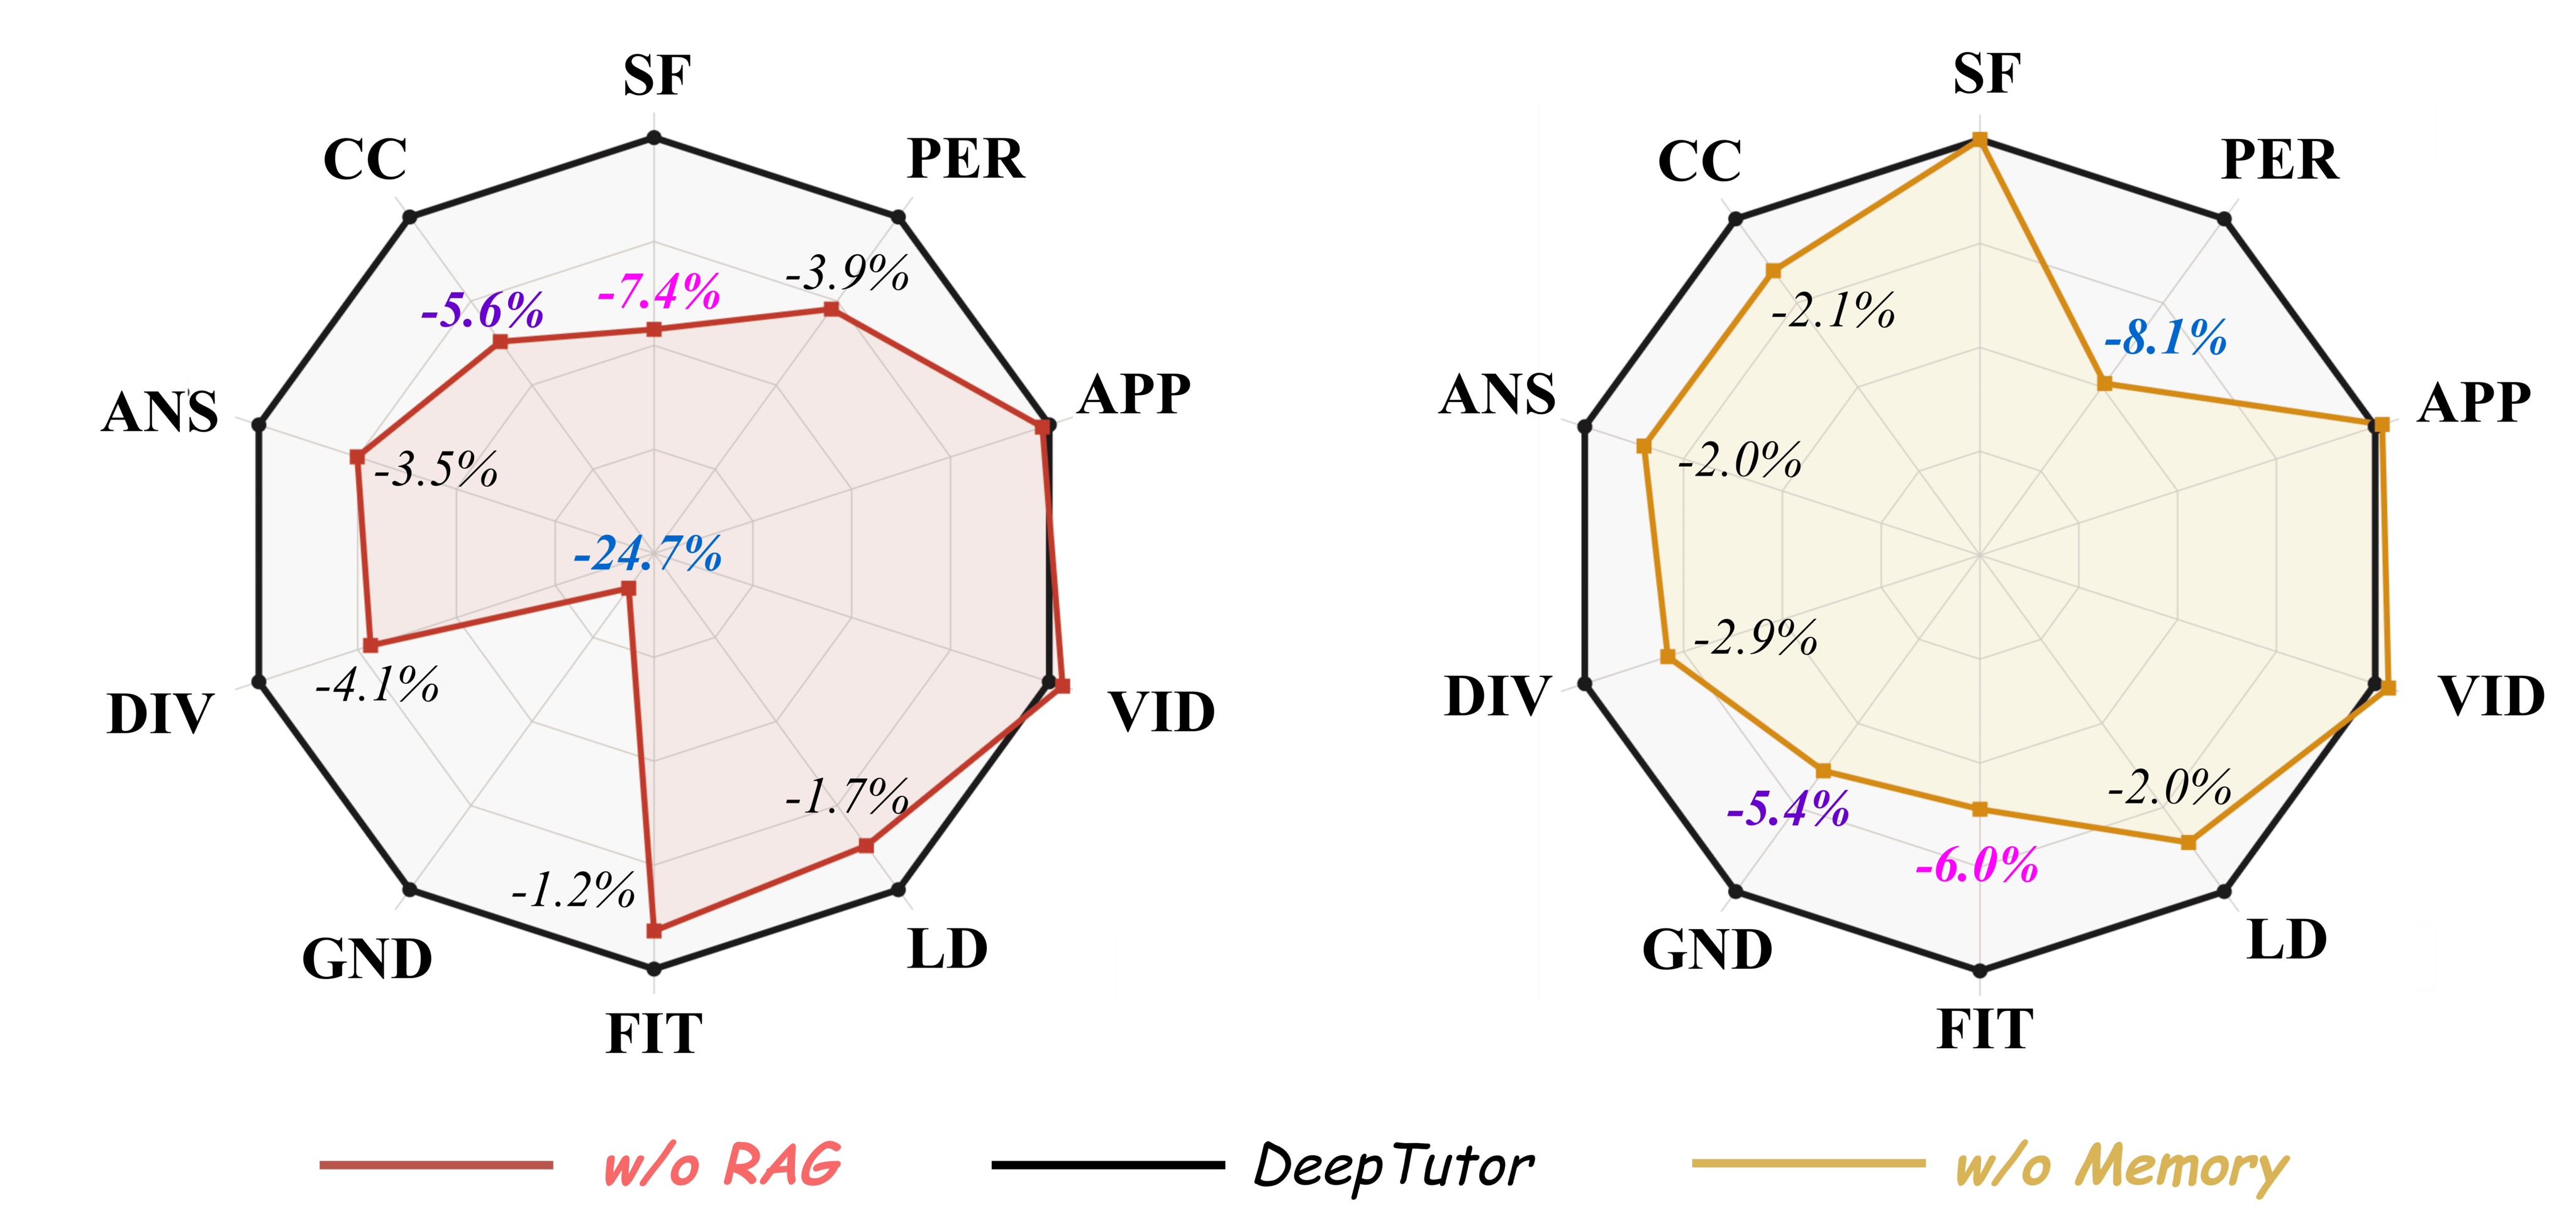
\includegraphics[width=\columnwidth]{figures/ablation-0316.png}
  \caption{Per-metric impact of removing RAG (left) and Memory (right). Black decagon: full \textsc{DeepTutor}; shaded region: ablated variant. Labels highlight the three largest drops (\textcolor[RGB]{39,123,255}{1st}, \textcolor[RGB]{255,74,234}{2nd}, \textcolor[RGB]{147,92,255}{3rd}).}
  \label{fig:ablation_radar}
\end{figure}

We ablate RAG, Memory, or both from the full pipeline (lower block of Table~\ref{tab:interactive_all}, visualized in Figure~\ref{fig:ablation_radar}).

\textbf{Removing RAG} primarily erodes content-grounding metrics.
\emph{Groundedness} suffers the steepest decline ($-$0.73), followed by \emph{Source Faithfulness} and \emph{Cross Concept}.
This is expected: without retrieval, the system loses access to the authoritative material that anchors both explanations and practice items.

\textbf{Removing Memory} instead compresses the personalization cluster.
\emph{Personalization} falls most sharply ($-$0.37), followed by \emph{Fitness} and \emph{Groundedness}.
The drop in \emph{Fitness} is particularly informative, as it confirms that learner memory is the primary signal for calibrating practice difficulty to the individual.

The two ablation patterns contract along \emph{largely complementary} axes: RAG governs \emph{what} the tutor says in terms of factual grounding, while Memory shapes \emph{how} it adapts in terms of personalization depth.
This complementarity confirms that the two components serve distinct functions and reinforces the rationale behind the hybrid personalization engine.
Even when both are removed, \textsc{DeepTutor} still outperforms all baselines by 4.82\%, indicating that the multi-stage pipeline itself contributes meaningfully beyond the personalization modules.

% ============================================================
\section{Conclusion}
\label{sec:conclusion}
% ============================================================

In this paper, we present \textsc{DeepTutor}, an open-source framework for personalized tutoring built around a shared personalization substrate and organized along two complementary dimensions.

The first dimension, \emph{personalized agentic tutoring}, establishes the validated core of the system.
A hybrid personalization engine couples static knowledge grounding with a dynamic trace forest to close a bidirectional loop between citation-grounded problem solving and difficulty-calibrated question generation.
The same engine extends to collaborative writing, deep research, and guided learning, ensuring that progress in any modality informs the others.
The second dimension, \emph{proactive autonomous companionship}, deploys these capabilities in a broader setting through TutorBot, where autonomous agents operate through extensible skills, multi-bot coordination, and context-unified multi-channel access.

Evaluation of the foundational pipeline on TutorBench, together with a first-person interactive protocol designed from the learner's perspective, demonstrates a 10.8\% improvement on personalized tutoring metrics and an average 28.6\% gain on general reasoning benchmarks across five backbone models.
Ablation studies confirm that knowledge grounding and learner memory contribute along largely complementary axes, validating the hybrid design upon which the broader system is built.

\paragraph{Broader Implications.}
The architectural pattern explored here extends beyond education.
Whenever an AI system must personalize over time while remaining coherent across tools and interfaces, a shared personalization substrate paired with a proactive deployment layer offers a useful design template.
\textsc{DeepTutor} can be viewed as one concrete instantiation of this broader class of agentic personalized systems.

\paragraph{Future Work.}
Longitudinal deployment studies with real students would provide the most rigorous validation of the cognitive extensions and the proactive multi-agent layer.
Collaborative writing, deep research, guided learning, and cross-channel TutorBot behaviors should be evaluated with deployment-scale metrics that capture retention, follow-up quality, and sustained learner engagement.
The trace forest could benefit from more sophisticated consolidation strategies, such as importance-weighted compression and cross-modality summarization, as interaction histories grow over time.
Integrating multimodal understanding of handwriting, diagrams, and speech would further close the gap between AI-based and human tutoring.
Finally, formalizing the conditions under which proactive agency improves learning outcomes, rather than merely system capability, remains an important open question for the community.

\section*{Limitations}

Our interactive evaluation relies on LLM-powered student simulators and rubric-based assessors, which inherit an irreducible gap between controlled simulation and real learner behavior.
Large-scale validation with human students is an essential next step.
For reasons of experimental tractability and evaluation cost, this report concentrates quantitative study on the foundational tutoring pipeline rather than attempting to fully measure every higher-level modality and proactive behavior in a single benchmark.
The general reasoning evaluation in Table~\ref{tab:generalization} compares the full pipeline, including its tool suite, against bare backbone models; isolating the contribution of the pipeline structure alone from the contribution of tool augmentation requires further experimentation.
The multi-stage pipeline trades additional inference cost for stronger controllability and personalization, and the economics of this trade-off depend on the deployment context.
Evaluation of the cognitive extensions and TutorBot requires longitudinal and deployment-based studies that remain future work.
The TutorBench construction pipeline could be extended to finer-grained courses, longer trajectories, and more diverse populations.
While we articulate a design for context-unified proactive tutoring, rigorously measuring its long-term impact on learning outcomes remains an open frontier.


\bibliographystyle{plainnat}
\bibliography{references}

\appendix
% =============================================================================
% Appendix
% =============================================================================

\section{System Algorithms}
\label{app:algorithms}

This appendix provides complete pseudocode for the two core algorithmic loops that drive \textsc{DeepTutor}: the closed-loop personalized tutoring cycle~(\S\ref{app:algorithm}) and the TutorBot autonomous agent loop~(\S\ref{app:tutorbot}).

\subsection{Closed-Loop Tutoring}
\label{app:algorithm}

Algorithm~\ref{alg:loop} provides the complete pseudocode for the closed-loop personalized tutoring cycle described in \S\ref{sec:cycle}.
At the start of each session, the personalization engine injects the current learner profile and relevant traces into the working context.
Depending on the task type, the pipeline dispatches to either the three-stage problem-solving path (Stages~\ding{172}--\ding{174}) or the two-stage question-generation path (Stages~\ding{175}--\ding{176}).
After every interaction, the resulting trace is appended to the forest and the three memory agents update the learner profile in parallel.

\begin{algorithm}[ht!]
\caption{Closed-Loop Personalized Tutoring}\label{alg:loop}
\small
\begin{algorithmic}[1]
\Require learner profile $\mathcal{D}^{(0)}$;\; trace forest $\mathcal{F}^{(0)} = \emptyset$
\For{session $j = 1, 2, \ldots$}
    \State $\mathcal{C}_{\text{mem}} \gets \Call{ProfileInject}{\mathcal{D}^{(j{-}1)}, \mathcal{F}^{(j{-}1)}, \text{task}_j}$
    \If{$\text{task}_j = (\textsc{Solve},\, q)$}
        \State $\mathcal{C}_{\text{rag}} \gets \textsc{RagTool}(q)$
        \State $\mathcal{E}_{\text{plan}} \gets \Call{Investigate}{q,\;\mathcal{C}_{\text{rag}},\;\mathcal{C}_{\text{mem}},\;\mathcal{F}^{(j{-}1)}}$ \Comment{\ding{172}}
        \State $\mathcal{P}{=}\langle s_1,\dots,s_K\rangle \gets \Call{Plan}{q,\;\mathcal{E}_{\text{plan}},\;\mathcal{C}_{\text{mem}}}$
        \For{$k = 1$ \textbf{to} $K$} \Comment{\ding{173}}
            \While{$s_k$ not resolved}
                \State $(\alpha_t,\, \mathbf{s}_t) \gets \Call{ToolAgent}{q, \mathcal{P}, \mathcal{S}, \mathcal{C}_{\text{rag}}, \mathcal{C}_{\text{mem}}}$
                \State $\mathcal{S} \gets \mathcal{S} \cup \{\mathbf{s}_t\}$
                \If{$\alpha_t = \textsc{Replan}$}
                    \State $\mathcal{P} \gets \Call{Revise}{\mathcal{P}, \mathcal{S}}$
                \EndIf
            \EndWhile
            \State $\mathcal{S} \gets \Call{Compress}{\mathcal{S}, k}$
        \EndFor
        \State $a \gets \Call{IterativeWrite}{\mathcal{S},\;\mathcal{C}_{\text{mem}}}$ \Comment{\ding{174}}
        \State $T_j \gets \Call{BuildTrace}{q, a}$
    \Else \Comment{$\text{task}_j = (\textsc{Generate},\, \tau)$}
      \State $\mathcal{C}_{\text{rag}} \gets \textsc{RagTool}(\tau)$
        \State $f_{\text{idea}} \gets \emptyset$
        \Repeat
            \State $\mathcal{I} \gets \Call{IdeaAgent}{\tau,\;\mathcal{C}_{\text{rag}},\;\mathcal{C}_{\text{mem}},\;f_{\text{idea}}}$ \Comment{\ding{175}}
            \State $(\textit{continue},\, f_{\text{idea}},\, \mathcal{T}_{1..N}) \gets \Call{EvaluateIdeas}{\mathcal{I},\;\tau,\;\mathcal{C}_{\text{mem}}}$
        \Until{$\lnot\,\textit{continue}$}
        \For{$i = 1$ \textbf{to} $N$} \Comment{\ding{176}}
            \Repeat
                \State $(q_i, a_i) \gets \Call{Generator}{\mathcal{T}_i,\;\mathcal{C}_{\text{rag}},\;\mathcal{C}_{\text{mem}}}$
                \State $(\textit{pass}, f_i) \gets \Call{Validator}{q_i, a_i, \mathcal{T}_i}$
                \If{$\lnot\,\textit{pass}$} $\mathcal{T}_i \gets \Call{Revise}{\mathcal{T}_i, f_i}$
                \EndIf
            \Until{\textit{pass}}
        \EndFor
        \State $T_j \gets \Call{BuildTrace}{\tau, \{(q_i, a_i)\}}$
    \EndIf
    \State $\mathcal{F}^{(j)} \gets \mathcal{F}^{(j{-}1)} \cup \{T_j\}$
    \State $\mathcal{D}^{(j)} \gets \Call{MemoryUpdate}{\mathcal{D}^{(j{-}1)}, T_j}$
\EndFor
\end{algorithmic}
\end{algorithm}

% ============================================================
\subsection{TutorBot Autonomous Agent Loop}
\label{app:tutorbot}
% ============================================================

Algorithm~\ref{alg:tutorbot} provides the pseudocode for the TutorBot autonomous agent loop described in \S\ref{sec:agentloop}.
Each inbound message triggers a three-phase cycle: context assembly, iterative tool-augmented reasoning, and memory consolidation.
The \textsc{BuildContext} procedure weaves the bot's persona (Soul), long-term memory, skill descriptions, and conversation history into a single prompt.
The inner ReAct loop calls the LLM, executes any requested tools, and appends results until a final response is produced or the iteration budget is exhausted.
After each turn, the memory consolidator checks whether the accumulated history exceeds half the context window; if so, it distills the oldest unconsolidated messages into the two-layer persistent memory (long-term profile and session history log), advancing the consolidation pointer to reclaim context space for future turns.

\begin{algorithm}[ht!]
\caption{TutorBot Autonomous Agent Loop}\label{alg:tutorbot}
\small
\begin{algorithmic}[1]
\Require message bus $\mathcal{B}$;\; LLM provider $\mathcal{M}$;\; tool registry $\mathcal{T}$;\; session store $\mathcal{S}$;\; context window $W$;\; max iterations $I_{\max}$
\Statex
\Loop \Comment{Main event loop}
    \State $m \gets \mathcal{B}.\textsc{ConsumeInbound}()$ \Comment{Block until next message}
    \State $\sigma \gets \mathcal{S}.\textsc{GetOrCreate}(m.\textit{session\_key})$
    \Statex
    \Comment{\textbf{Phase 1: Context Assembly}}
    \State $\textit{sys} \gets \textsc{BuildContext}(\sigma.\textit{soul},\; \sigma.\textit{memory},\; \sigma.\textit{skills})$
    \State $H \gets \sigma.\textsc{GetHistory}()$ \Comment{Unconsolidated messages}
    \State $\textit{msgs} \gets [\textit{sys}] \,\|\, H \,\|\, [\textsc{Wrap}(m)]$
    \Statex
    \Comment{\textbf{Phase 2: ReAct Tool-Calling Loop}}
    \For{$i = 1$ \textbf{to} $I_{\max}$}
        \State $r \gets \mathcal{M}.\textsc{Chat}(\textit{msgs},\; \mathcal{T}.\textsc{Definitions}())$
        \If{$r$ has no tool calls}
            \State $\textit{response} \gets r.\textit{content}$ \Comment{Final answer}
            \State \textbf{break}
        \EndIf
        \State Append assistant message (with tool calls) to $\textit{msgs}$
        \ForAll{tool call $\tau$ in $r.\textit{tool\_calls}$}
            \State $\textit{result} \gets \mathcal{T}.\textsc{Execute}(\tau.\textit{name},\; \tau.\textit{args})$
            \State Append tool result to $\textit{msgs}$
        \EndFor
    \EndFor
    \Statex
    \Comment{\textbf{Phase 3: Persist \& Consolidate}}
    \State $\sigma.\textsc{AppendTurn}(\textit{msgs})$
    \If{$\textsc{EstimateTokens}(\sigma) > W$} \Comment{Context pressure}
        \State $\textit{chunk} \gets \sigma.\textit{messages}[\sigma.\textit{ptr} : \textit{boundary}]$
        \State $\textsc{Consolidate}(\textit{chunk},\; \sigma.\textit{memory})$ \Comment{LLM-based distillation}
        \State $\sigma.\textit{ptr} \gets \textit{boundary}$
    \EndIf
    \State $\mathcal{S}.\textsc{Save}(\sigma)$
    \State $\mathcal{B}.\textsc{PublishOutbound}(\textit{response},\; m.\textit{channel})$
\EndLoop
\end{algorithmic}
\end{algorithm}

The \textsc{BuildContext} procedure constructs the system prompt by concatenating the following components in order:
(1)~the bot's core identity and runtime metadata,
(2)~bootstrap files including the Soul template (persona), user preferences, and tool guidelines,
(3)~long-term memory (user profile and learning context summaries),
(4)~always-active skill descriptions, and
(5)~a summary of all available skills for on-demand loading.
The \textsc{Consolidate} procedure invokes the LLM with a dedicated ``memory consolidation agent'' system prompt, forcing a structured tool call that produces both a timestamped history entry (appended to the session log) and an updated long-term profile (overwriting the previous version).
This two-output design ensures that consolidation simultaneously preserves searchable event detail and maintains a concise, current learner model.

% ============================================================
\section{Extended Evaluation Details}
\label{app:eval}
% ============================================================

\subsection{Evaluation Rubrics}
\label{app:eval:rubrics}

Each of the ten metrics is evaluated on a 1--5 Likert scale by an LLM judge.
Below we provide the defining criteria for each metric.

\paragraph{Solve-Side Metrics.}
\begin{itemize}[nosep,leftmargin=*]
\item \textbf{Source Faithfulness~(SF)}: factual consistency with the source material, terminological precision, grounding in retrieved evidence, and explicit source attribution.
\item \textbf{Personalization~(PER)}: tailoring to the specific learner's diagnosed misunderstandings and conversational trajectory.
\item \textbf{Applicability~(APP)}: provision of concrete, immediately actionable guidance.
\item \textbf{Vividness~(VID)}: richness of multimodal delivery elements (examples, analogies, structured formatting) that enhance understanding.
\item \textbf{Logical Depth~(LD)}: presence of explicit, multi-step causal reasoning chains.
\end{itemize}

\paragraph{Practice-Side Metrics.}
\begin{itemize}[nosep,leftmargin=*]
\item \textbf{Fitness~(FIT)}: alignment with session-level diagnosed weaknesses at an appropriate difficulty level.
\item \textbf{Groundedness~(GND)}: factual anchoring in the source material.
\item \textbf{Diversity~(DIV)}: novelty in angle and cognitive demand across generated questions.
\item \textbf{Answer Quality~(ANS)}: correctness of the answer key and plausibility of distractors.
\item \textbf{Cross Concept~(CC)}: meaningful integration of multiple concepts within a single question.
\end{itemize}

\subsection{Student Simulator}
\label{app:eval:simulator}

\begin{figure*}[t]
    \centering
    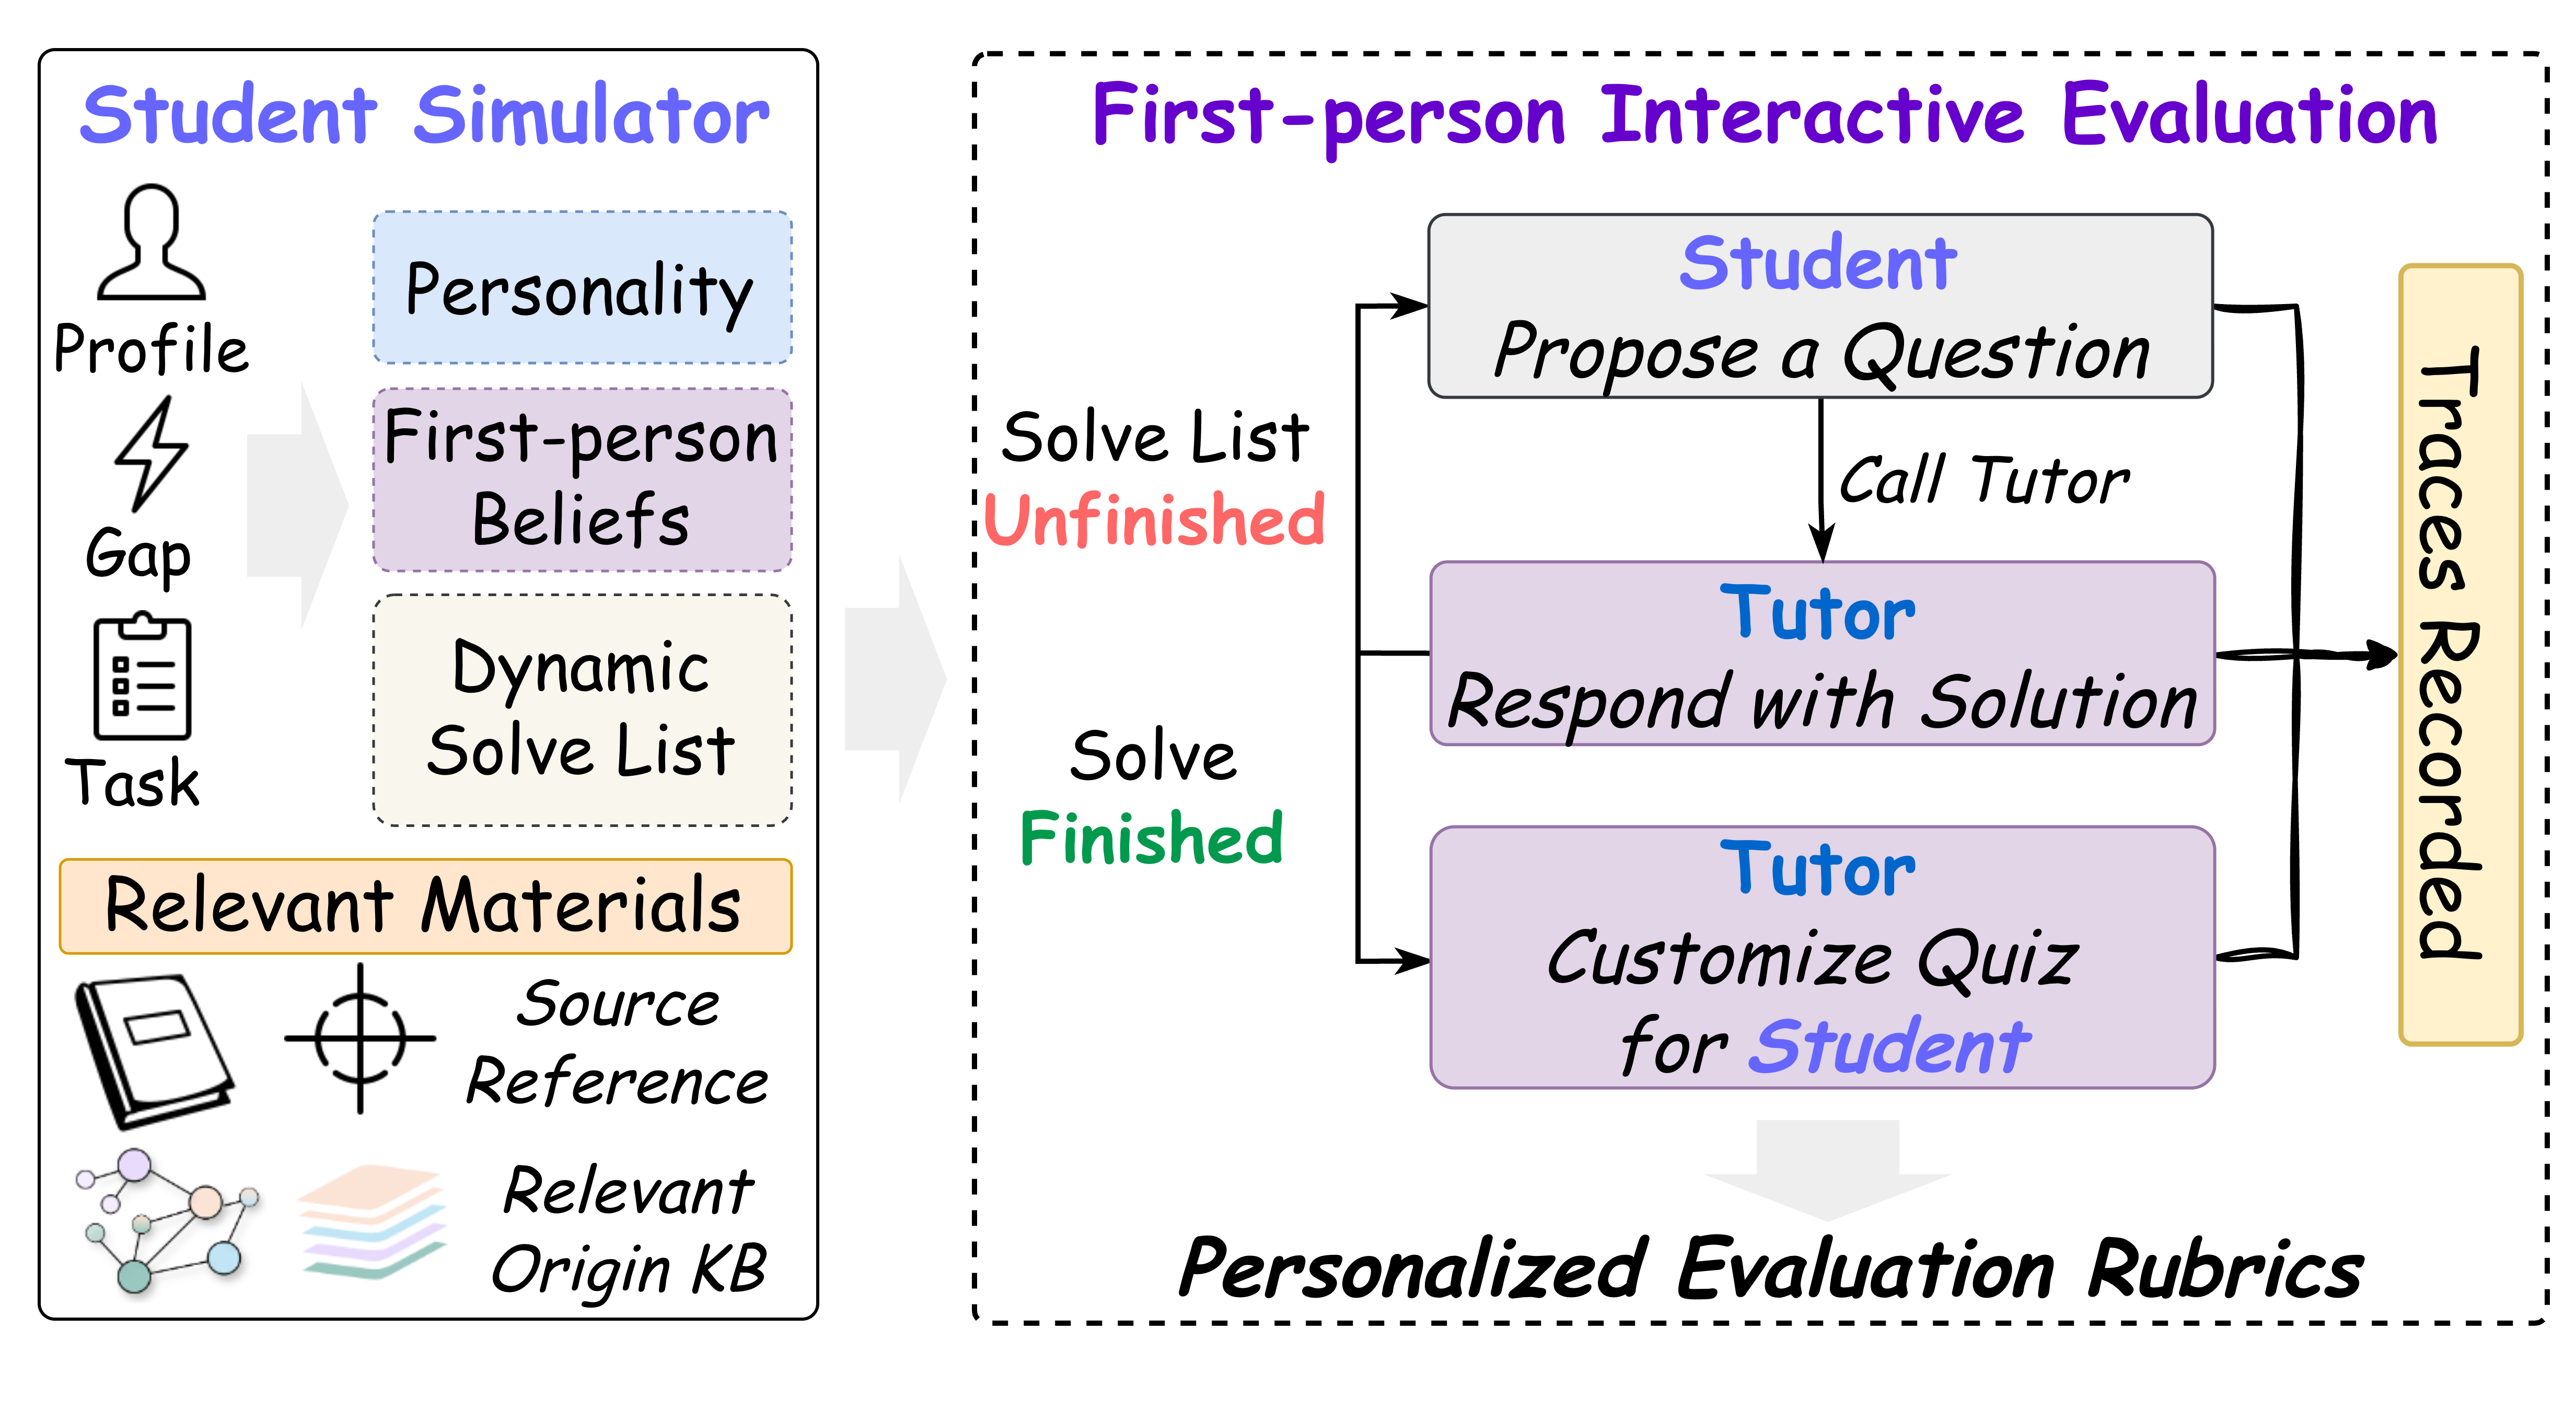
\includegraphics[width=\textwidth]{figures/eval-0315.png}
    \caption{First-person interactive evaluation protocol. A student simulator initialized from a \textsc{TutorBench} entry engages the tutoring system in multi-turn dialogue; the resulting transcript is scored against a personalized rubric by an independent judge.}
    \label{fig:evaluation}
\end{figure*}

The student simulator is an LLM agent initialized from a \textsc{TutorBench} entry comprising a learner profile, knowledge gaps, and an interactive task.
Each gap is pre-transformed into a first-person belief statement so that the simulator \emph{acts as} the student rather than narrating errors from an external perspective.
Listing~\ref{lst:simulator} gives the system prompt governing simulator behavior; template variables are populated from the entry at initialization time.

\begin{lstlisting}[caption={Student Simulator System Prompt},label={lst:simulator}]
You are role-playing as a student seeking help from an AI
tutor. Stay in character throughout the entire conversation.

# Who You Are
{personality}

# Your Background
{education_background}

# Why You Are Here
{learning_purpose}

# What You Know
You are confident about these topics:
{known_well}

You have vague or partial understanding:
{partially_known}

You have NO knowledge of the following:
{unknown}

# What You Believe (IMPORTANT -- these feel true to you)
{beliefs}

# Behavioral Rules
1. NEVER display knowledge listed as "unknown".
2. When the tutor teaches something new, try to rephrase
   it in your own words. It's okay to rephrase imperfectly.
3. If the tutor asks "do you understand?", be honest based
   on whether the explanation addressed your confusion.
4. Keep responses concise: 1-4 sentences typically.
5. Stay consistent with your personality throughout.
6. You may ask follow-up questions or request examples.
7. When you feel you've understood, PREFER asking for a
   practice problem before ending.

# Ending the conversation (ONLY when done)
Use [ACTION: task_complete] ONLY if ALL conditions are true:
- You are explicitly done.
- You have zero remaining questions.
- You are NOT requesting anything else.
- Your message is a natural closing/goodbye.
\end{lstlisting}

\paragraph{Dynamic Gap Pacing.}
The \texttt{\{beliefs\}} placeholder is populated with first-person formulations of each knowledge gap (e.g., ``I think the Poynting vector always points in the direction of wave propagation'').
The simulator's behavioral rules enforce realistic resistance patterns: the student may defend misconceptions, partially accept corrections, and only signal completion after sufficient scaffolded explanation.
This prevents trivially short sessions where the student immediately agrees with any tutor statement.

\subsection{Baseline Definitions}
\label{app:eval:baselines}

All baselines share the same backbone (\emph{Gemini-3-Flash}) and knowledge-base access as \textsc{DeepTutor}.
Each baseline receives the student's question together with the top-$k$ RAG-retrieved passages and a tutoring-oriented system prompt; they differ only in the reasoning strategy applied before producing the final response.

\paragraph{Notation.}
All baseline algorithms share the following primitives:
$\textsc{Rag}(m, K, \textit{mode}, k)$ retrieves $k$~passages from knowledge base~$K$ for query~$m$;
$\textsc{Concat}(\cdot)$ concatenates its arguments into a single context string; and
$\textsc{Llm}(p, H, \textit{ctx})$ denotes one LLM generation call with system prompt~$p$, conversation history~$H$, and user-side context~\textit{ctx}.

\paragraph{Naive Tutor.}
The simplest baseline: a single LLM call maps the concatenation of the system prompt, RAG context, and user question directly to a response.
No intermediate reasoning, self-critique, or tool use is involved.

\begin{algorithm}[ht!]
\caption{Naive Tutor}\label{alg:naive}
\small
\begin{algorithmic}[1]
\Require Student message $m$, history $H$, knowledge base $K$
\Statex \textbf{Prompt:} $p_{\text{tutor}}$ (tutoring persona)
\State $r_{\text{rag}} \gets \textsc{Rag}(m, K, \textit{naive}, k{=}2)$
\State $\textit{ctx} \gets \textsc{Concat}(r_{\text{rag}}, m)$
\State $\textit{response} \gets \textsc{Llm}(p_{\text{tutor}}, H, \textit{ctx})$
\State \Return \textit{response}
\end{algorithmic}
\end{algorithm}

\paragraph{CoT Tutor.}
Identical to the Naive Tutor except that the system prompt appends an explicit chain-of-thought directive~\citep{wei2022chain}, instructing the model to ``think step by step'' before answering.
The reasoning trace and the final answer are produced in one LLM call.

\begin{algorithm}[ht!]
\caption{CoT Tutor}\label{alg:cot}
\small
\begin{algorithmic}[1]
\Require Student message $m$, history $H$, knowledge base $K$
\Statex \textbf{Prompt:} $p_{\text{cot}}$ (tutoring persona + chain-of-thought directive)
\State $r_{\text{rag}} \gets \textsc{Rag}(m, K, \textit{naive}, k{=}2)$
\State $\textit{ctx} \gets \textsc{Concat}(r_{\text{rag}}, m)$
\State $\textit{response} \gets \textsc{Llm}(p_{\text{cot}}, H, \textit{ctx})$
\State \Return \textit{response}
\end{algorithmic}
\end{algorithm}

\paragraph{Self-Refine Tutor.}
A two-pass pipeline inspired by~\citet{madaan2024selfrefine}.
In the first pass, the model generates an initial draft answer.
In the second pass, a pedagogical review prompt asks the same model to critique the draft for factual accuracy, personalization, and clarity, then produce a revised response.

\begin{algorithm}[ht!]
\caption{Self-Refine Tutor}\label{alg:selfrefine}
\small
\begin{algorithmic}[1]
\Require Student message $m$, history $H$, knowledge base $K$
\Statex \textbf{Prompts:} $p_{\text{tutor}}$ (tutoring persona), $p_{\text{ref}}$ (pedagogical reviewer)
\State $r_{\text{rag}} \gets \textsc{Rag}(m, K, \textit{naive}, k{=}2)$
\State $\textit{ctx} \gets \textsc{Concat}(r_{\text{rag}}, m)$
\State $\textit{draft} \gets \textsc{Llm}(p_{\text{tutor}}, H, \textit{ctx})$ \Comment{initial response}
\State $\textit{ctx}' \gets \textsc{Concat}(r_{\text{rag}}, m, \textit{draft})$
\State $\textit{response} \gets \textsc{Llm}(p_{\text{ref}}, H, \textit{ctx}')$ \Comment{refine for clarity \& pedagogy}
\State \Return \textit{response}
\end{algorithmic}
\end{algorithm}

\paragraph{ReAct Tutor.}
A single-round ReAct-inspired loop~\citep{yao2023reactsynergizingreasoningacting} per student turn via four sequential LLM calls: $p_{\text{think}}$ diagnoses the student's need; $p_{\text{act}}$ decides on a tutoring action plan; $p_{\text{obs}}$ reviews the thought--action pair; and $p_{\text{tutor}}$ synthesizes the accumulated reasoning into a final response.
Relative to \textsc{DeepTutor}, this baseline does not include a multi-step planner, external tool execution beyond the shared naive RAG context, or cross-session memory.

\begin{algorithm}[ht!]
\caption{ReAct Tutor (single-round per turn)}\label{alg:react}
\small
\begin{algorithmic}[1]
\Require Student message $m$, history $H$, knowledge base $K$
\Statex \textbf{Prompts:} $p_{\text{think}},\; p_{\text{act}},\; p_{\text{obs}},\; p_{\text{tutor}}$
\State $r \gets \textsc{Rag}(m, K, \textit{naive}, k{=}2)$
\State $c_0 \gets \textsc{Concat}(r, H, m)$ \Comment{base context}
\State $\textit{th} \gets \textsc{Llm}(p_{\text{think}}, c_0)$ \Comment{diagnose need}
\State $\textit{act} \gets \textsc{Llm}(p_{\text{act}}, \textsc{Concat}(c_0, \textit{th}))$ \Comment{plan action}
\State $\textit{obs} \gets \textsc{Llm}(p_{\text{obs}}, \textsc{Concat}(c_0, \textit{th}, \textit{act}))$ \Comment{review}
\State $\textit{resp} \gets \textsc{Llm}(p_{\text{tutor}}, H, \textsc{Concat}(c_0, \textit{th}, \textit{act}, \textit{obs}))$
\State \Return \textit{resp}
\end{algorithmic}
\end{algorithm}

\subsection{General Problem-Solving Setup}
\label{app:eval:general}

Tables~\ref{tab:benchmarks} and~\ref{tab:backbones} summarize the benchmarks and backbone models used for the general problem-solving evaluation reported in \S\ref{sec:generalization}.
Note that several benchmarks are evaluated on subsets rather than the full release: HLE uses a fixed 500-question subset, LiveBench uses only the reasoning subset, and GAIA scores are reported per difficulty level (L1--L3).

\begin{table}[ht!]
\centering
\small
\begin{tabular}{@{}llcc@{}}
\toprule
\textbf{Benchmark} & \textbf{Category} & \textbf{Size} & \textbf{Format} \\
\midrule
HLE~\citep{phan2025hle} & STEM reasoning & 500$^\dagger$ & open-ended \\
GPQA-Diamond~\citep{rein2024gpqa} & STEM reasoning & 198 & 4-choice MCQ \\
LiveBench~\citep{white2025livebench} & reasoning & subset$^\dagger$ & mixed \\
GAIA~\citep{mialon2024gaia} & agentic & 165 & open-ended \\
AA-LCR~\citep{artificialanalysis2025lcr} & long-context & 100 & open-ended \\
\bottomrule
\end{tabular}
\caption{Public benchmarks used in the general problem-solving evaluation.
$^\dagger$HLE uses a fixed 500-question subset; LiveBench uses the reasoning subset only.}
\label{tab:benchmarks}
\end{table}

All five backbone models are accessed via API.
Qwen-3.5-Plus is called through Alibaba Cloud (DashScope); the remaining four models are called through OpenRouter.
Table~\ref{tab:backbones} lists the exact model identifiers used.

\begin{table}[ht!]
\centering
\small
\begin{tabular}{@{}llll@{}}
\toprule
\textbf{Backbone} & \textbf{API Source} & \textbf{Model Name} & \textbf{Context} \\
\midrule
Gemini-3-Flash  & OpenRouter    & \texttt{google/gemini-3-flash}       & 1M \\
Sonnet-4.5      & OpenRouter    & \texttt{anthropic/claude-sonnet-4.5} & 200K \\
Qwen-3.5-Plus   & Alibaba Cloud & \texttt{qwen-plus}                  & 128K \\
GPT-5-Mini      & OpenRouter    & \texttt{openai/gpt-5-mini}           & 128K \\
Minimax-M2.5    & OpenRouter    & \texttt{minimax/minimax-m2.5}        & 1M \\
\bottomrule
\end{tabular}
\caption{Backbone models and API sources for the general problem-solving evaluation.}
\label{tab:backbones}
\end{table}

\paragraph{Evaluation Protocol.}
Correctness is assessed via a two-stage pipeline.
\emph{Stage~1 (Extract)}: an LLM extracts the model's final answer from its free-form output (model: Claude Sonnet~4.6, temperature~$= 0.0$, max tokens~$= 16\,384$).
\emph{Stage~2 (Judge)}: a second LLM call compares the extracted answer to the ground truth using benchmark-specific rubrics (same model and settings for consistency).
For GAIA, exact-match is applied per difficulty level (L1--L3); for GPQA and HLE, option matching or text equivalence is applied.
All pass@1 scores are reported as percentages.

\paragraph{Pipeline Configuration.}
Table~\ref{tab:pipeline_config} lists the tool configuration for the \textsc{DeepTutor} pipeline on each benchmark.
The \texttt{done} and \texttt{replan} control signals are always available.

\begin{table}[ht!]
\centering
\small
\begin{tabular}{@{}lll@{}}
\toprule
\textbf{Benchmark} & \textbf{Tools Enabled} & \textbf{Max Tokens} \\
\midrule
HLE        & \texttt{code\_execute}, \texttt{reason}                & 16\,384 \\
GPQA-D     & \texttt{code\_execute}, \texttt{reason}                & 16\,384 \\
LiveBench  & \texttt{code\_execute}, \texttt{reason}                & 16\,384 \\
GAIA       & \texttt{code\_execute}, \texttt{reason}, \texttt{web\_search} & 16\,384 \\
AA-LCR     & \texttt{code\_execute}, \texttt{reason}                & 16\,384 \\
\bottomrule
\end{tabular}
\caption{Per-benchmark pipeline configuration. \texttt{done} and \texttt{replan} are always available. Temperature is $0.0$ across all benchmarks.}
\label{tab:pipeline_config}
\end{table}

% ============================================================
\section{Extended Experimental Results}
\label{app:results}
% ============================================================

\subsection{Cross-Domain Breakdown}

Table~\ref{tab:domain} decomposes \textsc{DeepTutor}'s interactive evaluation results by discipline.
Solve-side quality is remarkably stable across domains, while practice-side metrics show moderate variation reflecting the differing demands of question construction across fields.

{%
\setlength{\aboverulesep}{0pt}%
\setlength{\belowrulesep}{0pt}%
\renewcommand{\arraystretch}{1.18}%
\begin{table*}[ht!]
\centering
\small
\begin{tabular*}{\textwidth}{l @{\extracolsep{\fill}} ccccc g ccccc g c}
\toprule
& \multicolumn{6}{c}{\textbf{Solve Quality}}
& \multicolumn{6}{c}{\textbf{Practice Quality}}
& \\
\cmidrule(lr){2-7} \cmidrule(lr){8-13}
\textbf{Domain}
  & SF & PER & APP & VID & LD & \textit{Avg}
  & FIT & GND & DIV & ANS & CC & \textit{Avg}
  & OQ \\
\midrule
Humanities
  & 3.37 & 4.57 & 4.51 & 4.75 & 4.67 & 4.38
  & 3.13 & 2.89 & 3.58 & 3.94 & 3.12 & 3.33
  & 3.85 \\
Sciences
  & 3.69 & 4.66 & 4.69 & 4.80 & 4.63 & 4.49
  & 4.11 & 3.12 & 3.16 & 4.46 & 3.53 & 3.68
  & 4.09 \\
Engineering
  & 3.72 & 4.56 & 4.54 & 4.66 & 4.25 & 4.35
  & 3.42 & 3.14 & 3.53 & 4.36 & 3.47 & 3.58
  & 3.97 \\
Business
  & 3.66 & 4.58 & 4.80 & 4.93 & 4.69 & 4.53
  & 3.92 & 3.01 & 3.42 & 4.28 & 3.69 & 3.66
  & 4.10 \\
Research
  & 3.00 & 4.66 & 4.58 & 4.92 & 4.60 & 4.35
  & 3.57 & 3.11 & 3.52 & 3.57 & 3.11 & 3.37
  & 3.86 \\
\bottomrule
\end{tabular*}
\caption{Cross-domain breakdown of \textsc{DeepTutor}'s interactive evaluation results. Solve-side quality is broadly stable; practice-side metrics show moderate domain-dependent variation.}
\label{tab:domain}
\end{table*}
}

\subsection{Full Metric Breakdown}

Table~\ref{tab:ablation_full} provides the full per-metric breakdown for all baselines and \textsc{DeepTutor} variants, complementing the aggregated results in Table~\ref{tab:interactive_all}.

\begin{table*}[ht!]
\centering
\small
\setlength{\tabcolsep}{4pt}
\resizebox{\textwidth}{!}{%
\begin{tabular}{lcccccccccc}
\toprule
\textbf{Variant}
  & \textbf{SF}$\uparrow$ & \textbf{PER}$\uparrow$
  & \textbf{APP}$\uparrow$ & \textbf{VID}$\uparrow$
  & \textbf{LD}$\uparrow$
  & \textbf{FIT}$\uparrow$ & \textbf{GND}$\uparrow$
  & \textbf{DIV}$\uparrow$ & \textbf{ANS}$\uparrow$
  & \textbf{CC}$\uparrow$ \\
\midrule
\textbf{Naive Tutor}  & 3.2192 & 4.2406 & 4.4438 & 3.8895 & 3.9894 & 3.1978 & 2.4563 & 2.8267 & 3.8744 & 3.1200 \\
\textbf{CoT Tutor}  & 3.3395 & 4.2238 & 4.4709 & 3.8190 & 4.0096 & 3.1800 & 2.4978 & 2.7911 & 3.8120 & 3.0444 \\
\textbf{Self-Refine}  & 3.2785 & 4.2756 & \textbf{4.6090} & 3.9384 & 4.1414 & 3.1711 & 2.4911 & 2.8756 & 3.8844 & 2.9689 \\
\textbf{ReAct Tutor}  & 3.3472 & 4.3722 & 4.4023 & 3.7044 & 3.9598 & 3.1578 & 2.4667 & 2.7511 & \underline{3.9444} & 3.0667 \\
\midrule
\textsc{DeepTutor}  & \textbf{3.3641} & \textbf{4.5930} & 4.5638 & 4.8145 & \textbf{4.6079} & \textbf{3.3500} & \textbf{2.9600} & \textbf{3.4422} & \textbf{3.9767} & \textbf{3.3822} \\
w/o RAG    & 3.1057 & \underline{4.4091} & 4.5537 & \textbf{4.8316} & \underline{4.5348} & \underline{3.3055} & 2.2311 & 3.3022 & 3.8355 & 3.1911 \\
w/o Memory & \underline{3.3554} & 4.2243 & 4.5695 & \underline{4.8269} & 4.5156 & 3.1538 & \underline{2.8022} & \underline{3.3400} & 3.9011 & \underline{3.3089} \\
w/o Both  & 3.1609 & 4.1724 & \underline{4.5983} & 4.8200 & 4.4811 & 3.2533 & 2.2211 & 3.2733 & 3.8522 & 3.1356 \\
\bottomrule
\end{tabular}
}
\caption{Full per-metric breakdown across all baselines and \textsc{DeepTutor} variants. All values are 1--5 averages over the complete \textsc{TutorBench} evaluation set.}
\label{tab:ablation_full}
\end{table*}

% ============================================================
\section{TutorBench Construction Details}
\label{app:tutorbench}
% ============================================================

\subsection{Source Material Inventory}
\label{app:tutorbench:sources}

\textsc{TutorBench} is constructed from 30 knowledge bases derived from publicly available source materials.
For textbook sources, each book is partitioned into three chapter-contiguous segments; for research sources, each paper constitutes a single knowledge base.

\paragraph{Textbook-Derived Sources} (all from OpenStax):
\emph{Calculus Vol.~2} (Ch.~1--2, 3--4, 5--6),
\emph{Calculus Vol.~3} (Ch.~1--2, 3--4, 5--6),
\emph{Principles of Economics~3e} (Ch.~1--6, 7--12, 13--18),
\emph{Foundations of Information Systems} (Ch.~1--3, 4--6, 7--9),
\emph{Introduction to Computer Science} (Ch.~1--3, 4--6, 7--9),
\emph{Introduction to Philosophy} (Ch.~1--4, 5--8, 9--12),
\emph{Introduction to Business} (Ch.~1--5, 6--10, 11--15),
\emph{Writing Guide with Handbook} (Ch.~1--6, 7--12, 13--18).

\paragraph{Research Paper Sources:}
\emph{Memory in the Age of AI Agents}~\citep{hu2025memory},
\emph{DeepSeek-R1}~\citep{guo2025deepseekr1},
\emph{LiveCodeBench}~\citep{jain2025livecodebench},
\emph{OpenVLA}~\citep{kim2025openvla},
\emph{Towards the Reasoning Era}~\citep{chen2025towardsreasoningera},
\emph{YOLOv9}~\citep{wang2024yolov9}.

\subsection{Task Generation via Rejection Sampling}
\label{app:tutorbench:task}

Given a learner profile $p$ and its associated knowledge gaps $G$, the task generator creates interactive learning tasks distributed across four types:
\emph{concept understanding}~(30\%), \emph{problem solving}~(30\%), \emph{application}~(20\%), and \emph{comparison}~(20\%).
A rejection sampler filters candidate tasks on three criteria:
(1)~gap coherence, requiring each gap to be internally consistent and non-trivial;
(2)~task--gap alignment, requiring the task to naturally elicit the targeted gap;
and (3)~conversational naturalness, requiring the task to read as something a real student would plausibly ask.
The oracle applies strict acceptance criteria; when in doubt, it rejects.
This conservative stance accepts higher regeneration rates in exchange for higher task quality.



\end{document}
